% concatenated from Ikeda-Kouno-Naito.tex
%\documentclass[12pt]{article}
\documentclass[12pt,a4paper]{amsart}
\RequirePackage{iftex}

% arXiv(pdfLaTeX)ではPDFモードを強制（pLaTeXでは\pdfoutputが無いのでガード）
\ifdefined\pdfoutput
  \pdfoutput=1
\fi

% ドライバは「ロード前に」指定（\usepackage[...]{...}を混在させない）
\ifPDFTeX
  \PassOptionsToPackage{pdftex}{graphicx}
  \PassOptionsToPackage{pdftex}{xcolor}
\else
  % (u)pLaTeX + dvipdfmx
  \PassOptionsToPackage{dvipdfmx}{graphicx}
  \PassOptionsToPackage{dvipdfmx}{xcolor}
\fi

\usepackage{graphicx}
\usepackage{xcolor}
\usepackage{tikz}

\usepackage{amsmath,amsthm,mathtools, amsfonts,amssymb}%,showkeys}

\usepackage[utf8]{inputenc}
%\usepackage[dvipsnames]{xcolor}
% \usetikzlibrary{arrows.meta, decorations.markings, positioning}
%\usepackage[dvipdfmx]{graphicx,xcolor}
\usepackage{graphicx} % Required for inserting images
\usepackage{color}
\usepackage{xcolor}
\usepackage{tikz}
\usepackage{tikz-cd}
\usepackage[all]{xy}
\usetikzlibrary{cd,positioning}
\usepackage{hyperref}
\usepackage{extarrows}
\usepackage{ytableau}

\usepackage[mathscr]{euscript}

\usepackage[colorinlistoftodos]{todonotes}
\usepackage{amsmath}
\allowdisplaybreaks[4] 
\numberwithin{equation}{section}


%\documentclass[tikz,border=5pt]{standalone}
\usepackage{tikz}



\date{}

\newcommand{\Inv}{\mathrm{Inv}}
\newcommand{\Des}{\mathrm{Des}}
\newcommand{\G}{\mathfrak{G}}
\newcommand{\Gr}{\mathrm{Gr}}
\newcommand{\loc}{\mathrm{loc}}
\newcommand{\OGr}{\ell}
\newcommand{\F}{\mathbb{F}}
\newcommand{\ePet}{\hat{\mathbb{L}}_G}
\newcommand{\minrep}[1]{\lfloor #1\rfloor_P}
\newcommand{\Pet}{\mathbb{L}_G}
\newcommand{\Sc}{\mathfrak{S}}
\newcommand{\Z}{\mathbb{Z}}
\newcommand{\eps}{\varepsilon}
\newcommand{\SP}{\mathscr{SP}}
\newcommand{\hL}{\hat{\Lambda}}
\newcommand{\Rep}{\mathscr{R}}
\newcommand{\bO}{\mathbb{O}}
\newcommand{\Winf}{W_\infty}
\newcommand{\Winfgr}{\Winf^0}
\newcommand{\RR}{\mathscr{R}}


\newcommand{\piv}{\varpi^\lor}
\newcommand{\alv}{\alpha^\lor}
\newcommand{\CO}{\mathscr{O}_{G/B}}
\newcommand{\COPi}{\mathscr{O}_{G/P_i}}
\newcommand{\COP}{\mathscr{O}_{G/P}}
\newcommand{\C}{\mathbb{C}}
\newcommand{\af}{\mathrm{af}}

 \newcommand{\miw}[1]{v_{#1}}
% \newcommand{\miw}[1]{v_{#1}}
\newcommand{\ad}{\mathrm{ad}}
\newcommand{\tgq}[3]{\widetilde{gq}^{(#1)}_{#2}(y|#3)}
\newcommand{\Wexgr}{\hat{W}_\af^0}

\newcommand{\pair}[2]{\langle #1, #2 \rangle}
\DeclareMathOperator{\inv}{Inv}


\newtheorem{thm}{Theorem}[section]
\newtheorem{lem}[thm]{Lemma}
\newtheorem{prop}[thm]{Proposition}
\newtheorem{cor}[thm]{Corollary}
\newtheorem{conj}[thm]{Conjecture}
\newtheorem{guess}[thm]{Guess}
\newtheorem{example}[thm]{Example}

\newtheorem{defn}[thm]{Definition}
\theoremstyle{remark}
\newtheorem{remark}[thm]{Remark}
\title[Seidel product formula in equivariant quantum K-theory]{Seidel product formula in equivariant quantum $K$-theory of flag varieties}
\author{Takeshi Ikeda, Takafumi Kouno, Satoshi Naito}

\begin{document}
\begin{abstract}
We prove a Seidel product formula
for the torus-equivariant quantum $K$-theory of a generalized flag variety $G/P.$
This is a natural generalization of 
the corresponding results by Buch, Chaput, and Perrin for the cominuscule flag varieties.
Our proof is based on the $K$-theoretic Peterson isomorphism, due to Kato. We also use a version of the $K$-theoretic nil-Hecke algebra associated with the extended affine Weyl group, which was studied by Ikeda, Shimozono, and Yamaguchi. \end{abstract}
\maketitle

\section{Introduction}


% Let $G$ be a simple simply connected complex linear algebraic group and $T\subset G$ a maximal torus, and $B\supset T$ a Borel subgroup.
% The $T$-equivariant quantum $K$-theory $QK_T(G/B)=(R(T)[[Q]]\otimes_{R(T)}K_T(G/B), \star)$ of the flag variety $G/B$ is
% a deformation of the classical equivariant  $K$-theory $K_T(G/B)$
% with a deformation parameters $Q=(Q_1,\ldots,Q_r),$ and $R(T)$ is the representation ring of $T.$ $QK_T(G/B)$
% equipped with distingushed $R(T)[[Q]]$-basis $\{\CO^w\}$, called \emph{Schubert basis}. Our main result is a \emph{Seidel product formula} for 
% $QK_T(G/B).$
% This generalizes the work of Buch, Chaput, and Perrin \cite{BCP} in the non-equivariant quantum $K$-theory of the cominuscule flag varieties.
Let \(G\) be a simple, simply connected complex algebraic group. Fix a
maximal torus \(T\) of \(G\) and a Borel subgroup \(B\) of \(G\)
containing \(T\).
We study the $T$-equivariant quantum $K$-theory\footnote{Throughout the paper, $QK_T(G/B)$ denotes the polynomial version of equivariant quantum $K$-theory, after Anderson--Chen--Tseng \cite{ACT}.} $QK_T(G/B)$
of the flag
variety $G/B$.
The ring $QK_T(G/B)$ admits the Schubert basis $\{\CO^w\}$ indexed by the
Weyl group $W$.

Seidel's construction \cite{S} has played an important role in quantum
cohomology and quantum $K$-theory.
In quantum $K$-theory, Buch, Chaput, and Perrin \cite{BCP} proved a Seidel
product formula for cominuscule flag varieties.
More recently, Li, Liu, Song, and Yang \cite{LLSY} studied the Seidel
representation for Grassmannians by using curve neighbourhood.
On the other hand, Chaput, Manivel, and Perrin  \cite{CMP,CP} established the
corresponding formula in equivariant quantum cohomology for arbitrary
$G/P$.


The main purpose of this paper is to prove a Seidel product formula in
$T$-equivariant quantum $K$-theory for general flag varieties $G/B$.
Our proof is a direct application of Kato's $K$-theoretic Peterson
isomorphism \cite{Kato} together with the extended Peterson algebra of
Ikeda--Shimozono--Yamaguchi \cite{ISY}.
Using Kato's pushforward formula \cite{Kato2}, we further obtain the corresponding
Seidel product formula for $QK_T(G/P)$ for any parabolic subgroup
$P\subset G$.


% Let $G$ be a simple, simply connected, complex linear algebraic group, and let $T\subset G$ be a maximal torus and $B\supset T$ a Borel subgroup.
% We study the $T$-equivariant quantum $K$-theory\footnote{Throughout this paper, $QK_T(G/B)$ denotes the polynomial
% version of equivariant quantum $K$-theory, after Anderson--Chen--Tseng \cite{ACT}.} $QK_T(G/B)$
% of the flag variety $G/B$, which is a $Q$-deformation of $K_T(G/B)$ with quantum parameters $Q=(Q_1,\ldots,Q_r)$.
% Here $R(T)$ denotes the representation ring of $T$, and 
% $R(T)[Q]$ denote the polynomial ring 
% $R(T)[Q_,\ldots,Q_r].$
% The ring $QK_T(G/B)$ is equipped with a distinguished $R(T)[Q]$-basis ${\CO^w}$, called the \emph{Schubert basis}.

% Recent advances in quantum $K$-theory include the Seidel representation for Grassmannians studied by Li, Liu, Song, and Yang \cite{LLSY} and the Seidel product formula for cominuscule flag varieties, due to Buch, Chaput, and Perrin \cite{BCP}, whose key idea traces back to Seidel’s original construction \cite{S}.
% For the equivariant quantum cohomology, Chaput, Manivel, and Perrin \cite{CMP,CP} established the Seidel product formula\footnote{In \cite{CP}, the authors corrected the formula stated in \cite{CMP} and proved additional results.} in $QH_T^*(G/P)$, where $P$ is any parabolic subgroup of $G.$ Motivated by these developments, we prove a {Seidel product formula} for $QK_T(G/B)$.
% This result yields
% a similar result for $QK_T(G/P)$ for any parabolic subgroup $P$ by using Kato's pushforward  formula.
\subsection{Seidel classes}
% In the study of quantum Schubert calculus, the multiplication by a so-called Seidel class has been investigated by Buch, Chaput, and Perrin. Let us first briefly review the results in \cite{BCP}. 
% Let $G$ be a simply-connected simple linear algebraic group over $\C.$
Let $I$ denote the index set of the Dynkin nodes of $G$.
A Dynkin node  $i\in I$ of $G$ is called \emph{special} (or \emph{cominuscule}) 
if 
\begin{equation}
\langle \alpha,\piv_i\rangle\in \{0,1\}\quad \text{for all positive roots $\alpha$},
\label{eq:cominuscule}
\end{equation}
%\kouno{$\beta$ instead of $\alpha$?}
where $\piv_i$ is the fundamental coweight corresponding to $i\in I$ (see \S \ref{ssec:Sigma}, \S \ref{ssec:Seidel} for other aspects of special nodes). 
Let $W$ be the Weyl group generated by standard generators $s_i\;(i\in I)$ of
simple reflections. 
Let $P_i$ be the standard maximal parabolic subgroup associated with $I\setminus \{i\}.$ We consider  
an element $\miw{i}$ in Weyl group $W$ of $G$ defined by
% \ike{Inverse?}
\begin{equation*}
w_\circ= \miw{i}\,w_{P_i},
\end{equation*} where
$w_\circ$ and $w_{P_i}$ are the longest elements of $W$ and  
$W_{P_i}=\langle s_j\mid j\in I\setminus \{i\}\rangle,$ respectively. 
% The element $v_i$ is also the unique maximal element in the set $W^{P_i}$ of minimal representatives for $W/W_{P_i}$. 
We call $\miw{i}$ the \emph{Seidel element} corresponding to a special node $i$.

The class $\CO^{\miw{i}}$, for special $i$, is 
called a \emph{Seidel class} since it is related to 
the so-called Seidel representation of the fundemental group $\pi_1(G^\ad)$ of the group $G^\ad=G/Z(G)$ of adjoint type, where $Z(G)$ is the center of $G.$
The group $\pi_1(G^\ad)$ is isomorphic to the quotient group $\Sigma:=P^\lor/Q^\lor,$ where $P^\lor$ and $Q^\lor$ are the coweight lattice and the coroot lattce,  respectively.
\subsection{Seidel product formula for $QK_T(G/B)$}
There is a natural $W$-action on $QK_T(G/B)$, called the \emph{left action},
defined in the setting of the torus-equivariant quantum $K$-theory.
We refer to \cite[\S 8.3]{MNS} for details.
For \(u\in W\), we denote by \(u^L\) the corresponding ring automorphism of \(QK_T(G/B)\).
In particular, the action on the (opposite) Schubert basis is given by
\eqref{eq:W acts CO} below.


\begin{thm}\label{thm:main}
Let $i$ be a special (cominuscule) node of the Dynkin diagram of $G,$
and $\miw{i}$ the Seidel element corresponding to $i$. Then,  for any $w\in W,$ we have 
    $$
\CO^{\miw{i}}\cdot \miw{i}^L{\CO^w}=Q^{\piv_i-w^{-1}(\piv_i)}\CO^{\miw{i} w}
$$
 in torus-equivatiant quantum $K$-theory $QK_T(G/B)$. 
\end{thm}


This generalizes the cominuscule case  treated by Buch--Chaput--Perrin \cite{BCP}
to the full flag variety $G/B$.

\subsection{Parabolic case}
Let $P$ be a standard parabolic subgroup of $G$. 
% Denote its coroot lattice by $Q_P$. 
Let $I_P$ be the subset of $I$ corresponding to $P.$
Let $W_P=\langle s_j\mid  j\in I_P\rangle$
%\kouno{$\langle s_{j} \mid j \in I_{P}\rangle$} 
be the subgroup corresponding to $P$, and 
let $W^P$ denote the set of minimal-length coset representatives of $W/W_P$. For each $w\in W^P$ there is the Schubert class $\COP^w$ in $QK_T(G/P).$
For $w\in W$, let $\minrep{w}$ denote the unique element of $W^P$ such that $wW_P=\minrep{w}W_P.$
 For $\beta \in Q^\lor$, 
define 
\begin{equation*}
\minrep{\beta}
=
\beta - \sum_{j \in I_P}
\langle \varpi_j^\lor, \beta \rangle \, \alpha_j^\lor .
\end{equation*}
% Let $i\in I\setminus I_P$ be
% a special node.
% \ike{Check if the condition $i\in I\setminus I_P$ on $i$ is needed.} 
\begin{cor}\label{cor:P}
In $QK_T(G/P)$, we have
\begin{equation*}
\COP^{\minrep{\miw{i}}}\cdot \miw{i}^L{\COP^w}=Q^{\minrep{\piv_i-w^{-1}(\piv_i)}}\COP^{\minrep{\miw{i} w}}
\quad\text{for $w\in W^P.$}
\end{equation*}
 \end{cor}
This is the exact $K$-theoretic analogue of the Seidel product formula of
Chaput--Perrin \cite{CP}.
This corollary follows immediately from Theorem~\ref{thm:main} by applying Kato's
pushforward homomorphism
\[\pi_*:
QK_T(G/B)\longrightarrow QK_T(G/P)
\]
% \kouno{Is the notation $\pi_{\ast}$ appropriate? There are other notations $\pi_{i}$.}
% \ike{Feb 13. We can write the map is induced by $\pi:G/B\rightarrow G/P$.}
in equivariant quantum $K$-theory \cite{Kato2}.
In particular, in the cominuscule case $P=P_i$, this recovers the
non-equivariant formula of Buch--Chaput--Perrin \cite{BCP}.




% It is remarkable that the right hand side has only one term. In \cite{BCP}, some application of this formula including Pieri-type formula was derived. 


\subsection{$K$-theoretic Peterson isomorphism}

Our proof relies on the ``quantum equals affine'' philosophy, which goes
back to Peterson \cite{Pet}.

Let $\Gr_G$ be the affine Grassmannian of $G$.
The $T$-equivariant $K$-homology $K_*^T(\Gr_G)$ is equipped with the
Pontryagin product (see \cite{LSS,Kumar:conj}).
% \ike{Feb 19. I edited a little.}
A central ingredient is the $K$-theoretic Peterson isomorphism,
conjectured in \cite{LLMS} and established by Kato \cite{Kato}.
It yields an isomorphism of $R(T)$-algebras (see Theorem~\ref{thm:Kato})
\[
\Phi:
K_*^T(\Gr_G)_{\loc}\xrightarrow{\ \sim\ } QK_T(G/B)_{\loc}.
\]
Here the subscript $\loc$ indicates suitable localizations on both sides.




{\subsection{Extended $K$-theoretic Peterson algebra}

We also use an extended version of
the $K$-theoretic nil-Hecke algebra developed by
Ikeda--Shimozono--Yamaguchi \cite{ISY}.

Let $\hat{W}_{\af}=\Sigma\ltimes W_{\af}$ be the extended affine Weyl
group. In \cite{ISY}, an $R(T^{\ad})$-algebra $\hat{\mathbb{K}}_{\af}$ was constructed.
Inside $\hat{\mathbb{K}}_{\af}$, the authors define a commutative subalgebra
$\ePet$, called the extended $K$-theoretic Peterson algebra, which provides
an algebraic model for $K_*^{T^{\ad}}(\Gr_{G^{\ad}})$.
We refer to \cite{ISY} for precise definitions.
$\hat{\mathbb{K}}_{\af}$ acts on $\ePet$ naturally. 
This action incorporates the natural $\hat{W}_{\af}$-symmetry, in
particular the action of $\Sigma\simeq \pi_1(G^{\ad})$.
}


\subsection{Related works}
% \ike{Cite also Chow , Leung}
The 
Seidel product formula may be viewed as reflections of the hidden \emph{affine symmetry} of  Gromov-Witten invariants. Related symmetry phenomena in quantum Schubert calculus have been  investigated by several authors, including 
Chaput, Manivel, and Perrin \cite{CMP2010}, 
Agnihotri and Woodward \cite{AW}, 
Belkale \cite{B}, Postnikov \cite{P}.
% {\color{blue}
Rooted in Seidel’s original construction, related connections with affine Schubert calculus were studied by Chow in (equivariant) quantum cohomology \cite{C} and by Chow and Leung in quantum 
$K$-theory \cite{CL}.





 % The present paper grew out of an effort to find a polynomial representative of $\CO^{\miw{n}}$ in type $C_n$ within the Borel-type presentation of equivariant quantum $K$-theory due to Kouno and Naito \cite{KN}. While such a representative is not yet available in a satisfactory form, our main result implies that multiplication by $\CO^{\miw{n}}$ is governed by a simple rule. %{\color{lightgray}Consequently, the relevant structure constants can be computed algebraically without constructing an explicit polynomial representative.}

% The paper stems out of the attempt to 
% give a polynomial expression for $\CO^{w^{\min}_n}$ in type $C_n$ based on the Borel type 
% presentation of equivariant quantum $K$-theory by Kouno
% and Naito \cite{KN}. Although we have not succeeded in finding a good polynomial representative for it, the result in the present paper shows the multiplication by 
% $\CO^{w^{\min}_n}$ is quite simple, so we do not need the polynomial representative in order to compute the structure constants  algebraically. 

\subsection*{Organization}
The paper is organized as follows. In \S\ref{sec:ePet}, we review the extended $K$-Peterson algebra and its $K$-Peterson subalgebra, restricting ourselves to the minimal facts needed for the proof of the main theorem. In \S\ref{sec:proof}, we give the proof of our Seidel product formula, and its Corollary. In Appendix  \ref{sec:ePetA}, we present a review on the construction of the extended 
$K$-Peterson algebra.
Finally, in Appendix  \ref{sec:exa}, we illustrate the main results through several explicit examples.

% \subsection*{Acknowledgements}
% We thank Mark Shimozono for helpful discussions.  
\section{Extended K-theoretic Peterson algebra: Preliminaries}\label{sec:ePet}
We begin by reviewing the extended version of the 
$K$-theoretic Peterson algebra \cite{ISY,LSS}, restricting ourselves to the facts needed for the proof of the main result. Further details and additional constructions are deferred to Appendix \ref{sec:ePetA}.
Next, we recall the 
$K$-theoretic Peterson isomorphism,  due to Kato \cite{Kato}.  We also discuss some basic properties of the Seidel element 
$\miw{i}$ in \S \ref{sec:Seidel}. 
%We use $\tgq{n}{w}{b}$ introduced in [Brahma-I].

\subsection{Root systems}
Let $R$ be the root system of $(G,T)$. Let $G^\ad$ be the group of adjoint type associated with $R$. Let $I$ denote the Dynkin node sets. $P^\lor$ and $Q^\lor$ are the coweight lattice and coroot lattice,  respectively, with standard basis $\{\piv_i\mid i\in I\}$ and $\{\alpha_i^\lor\mid i\in I\}$
%\kouno{$\alpha_{i}^{\vee}$?} 
of the fundamental coweights, and the simple coroots, respectively.

%Fundamental group of $G^\ad$
\subsection{Extended affine Weyl group $\hat{W}_\af$}\label{ssec:Sigma}
Let $I_\af=I\cup\{0\}$ be the Dynkin node set of the untwisted affine type root system associated with the underlying root system $R.$
The extended affine Weyl group $\hat{W}_\af$ is generated by 
$\Sigma\cong P^\lor/Q^\lor$
and $W_\af=\langle s_i\mid i\in I_\af\rangle. $
 $\Sigma$ acts on the affine Dynkin node set $I_\af$ as automorphisms of the graph,  and for each special node $i$, there is a unique element in $\Sigma$ denoted by $\pi_i$, sending $0$ to $i$ 
(see %\cite[Ch.~6]{Kac}, 
\cite[\S 10.1]{LS:Acta}). 

Let $W_\af^0$ and $\hat{W}_\af^0$ be the set of affine Grassmannian elements for 
$W_\af$ and $\hat{W}_\af$,  respectively. We have $\hat{W}_\af^0=\Sigma \cdot W_\af^0.$
% \subsection{Extended level zero $K$-theoretic nil Hecke algebra }
\subsection{Extended $K$-theoretic Peterson algebra}
\label{ssec:Extended Pet}
% Let $\mathbb{K}_\af$ be the affine level zero $K$-theoretic nil-Hecke algebra due to Lam, Schilling, and Shimozono. This is a subring of the twisted 
% group ring $(\mathrm{Frac}\,R(T))[W_\af]$ of $W_\af$, where $W_\af$ acts 
% on $\mathrm{Frac}\,R(T)$ by 
Let $\Pet\subset \mathbb{K}_\af$ and $\ePet\subset \hat{\mathbb{K}}_\af$ be the $K$-theoretic Peterson subalgebra and
its extended version.
We refer the construction of these algebras to \cite{ISY}, however, we give a brief review in Appendix  \ref{sec:ePetA} below, for the reader's convenience. 
% $\Pet$ is defined to be the centralizer subalgebra of $R(T)$ in 
$\Pet$ is a commutative $R(T)$-algebra, while
$\ePet$ is a commutative
$R(T^\ad)$-algebra. 
% We refer \cite{LSS}, \cite{ISY} for the construction of these algebras. We follow
% the notation in \cite{ISY}.
 $\Pet$ has a basis $\OGr_{x}\;(x\in {W}_\af^0)$ as an $R(T)$-module, while  
$\ePet$ has a basis $\OGr_{x}\;(x\in \hat{W}_\af^0)$ as an $R(T^\ad)$-module. 
There is an action of $\hat{\mathbb{K}}_\af$ on $\ePet$ called the \emph{star action} (see \cite[\S 2.4]{ISY}). In particular, 
the Weyl group $W$, which can be considered as a subset of $\hat{\mathbb{K}}_\af$ acts on $\ePet$ by the star action.



% \begin{remark}
%      There is a natural surjective map $T\longrightarrow T^\ad$ yielding an injective ring homomorphism $R(T^\ad)\rightarrow R(T).$ The map, via the natural  identifications 
% $R(T)=\Z[P]$ and $R(T^{\ad})=\Z[Q]$, is  
% the natural inclusion 
% $\Z[Q]\hookrightarrow \Z[P]$ .
% \end{remark}

\begin{lem}[{\cite[Lemma 2.26, (2.61)]{ISY}}, cf. \cite{IIS}]
\label{lem:Sigma acts on L}
For $x\in \hat{W}_\af^0$ and  $\sigma=t_{\gamma_\sigma} u_\sigma\in \Sigma$,
with $\gamma_\sigma\in P^\lor$ and $u_\sigma\in W$, we have
\begin{equation}\label{eq:pi on ell}
\OGr_{\sigma x}=\OGr_\sigma( u_\sigma*\OGr_x),
\end{equation}
where $u_\sigma*\OGr_x$ denotes the the star action of $u_\sigma$ on $\OGr_x.$
In particular, for $\sigma,\sigma'\in \Sigma$, we have
\begin{equation}
\OGr_{\sigma\sigma'}=
% \sigma*\OGr_{\sigma'}=
\OGr_{\sigma}(u_{\sigma}*\OGr_{\sigma'}).
\label{eq: ell sigma sigma}
\end{equation}
\end{lem}
% \begin{example}
% Let $G=GL_n(\C).$
% Then $\pi_1(G)=\langle \tau\rangle \cong \Z.$
% We have
% \begin{align*}
% \tau *\OGr_{\tau^i}=
% \OGr_{\tau}u_{\tau}(\OGr_{\tau^i})=
% \OGr_{\tau^{i+1}.}
% \end{align*}
% For $i>0$, the element 
% $\OGr_{\tau^i}$ corresponds to $$\tilde{g}_{\tau^i}(y|b)=\Omega(b_1|y)\cdots \Omega(b_i|y),$$ and $u_\tau$ sends $b_i$ to $b_{i+1}$ with $b_{n+1}=b_1,$
% under the realization given in \cite{ISY}.
% The above equation is realized as 
% \begin{align*}\tau*\tilde{g}_{\tau^i}(y|b)
% &=
% \tilde{g}_{\tau}(y|b)
% u_\tau(\tilde{g}_{\tau^i}(y|b))\\
% &=\Omega(b_1|y)\cdot
% \Omega(b_2|y)\cdots\Omega(b_{i+1}|y)\\
% &=\tilde{g}_{\tau^{i+1}}(y|b).
% \end{align*}
% \end{example}


\begin{prop}[{\cite[Proposition 2.32]{ISY}}]\label{prop:t factor}
For anti-dominant $\gamma\in P^\lor$, 
and $x\in \hat{W}_\af^0$, we have
\begin{equation*}
\OGr_{xt_\gamma}=
\OGr_{x}\OGr_{t_\gamma}.
\end{equation*}
\end{prop}


For $i\in I,$
define $
\sigma_i=\ell_{t_{-\piv_i}}\in \ePet$.


\begin{lem}[{\cite[Lemma 2.30]{ISY}}]
\label{lem:W invariance of sigma}
For all $i\in I,$ $\sigma_i$ is invariant under the star action of $W.$ 
\end{lem}

\subsection{$K$-theoretic Peterson isomorphism }

For $w\in {W}$, let 
$\mathrm{Des}(w)
=\{i\in I\mid \OGr(ws_i)=\OGr(w)-1\},$
be the right descent set of $w$, 
and 
\begin{equation}
\gamma_w=-\sum_{j\in \Des(w)}\piv_j\in P^\lor.
\end{equation}
Then we have $wt_{\gamma_{x}} \in \hat{W}_{\af}$ (see \cite[Lemma 2.33]{ISY}).
For $w\in W$, define
% \kouno{How about mentioning that $wt_{\gamma_{x}} \in \hat{W}_{\af}$?}
% \ike{I did.}
the element
\begin{equation}
\bO^w:=
\frac{\OGr_{w t_{{\gamma_w}}}}{\OGr_{t_{{\gamma_w}}}}\in (\ePet)_{\loc}.
\end{equation}
\begin{prop} Let $w\in W$ and $\beta\in Q^\lor$ be anti-dominant so that 
$wt_\beta\in W_\af^0.$
Then 
\begin{equation*}
\frac{\OGr_{wt_\beta}}{\OGr_{t_\beta}}=\bO^w.
\end{equation*}
In particular, we have $\bO^w\in (\Pet)_{\loc}$.
\end{prop}
\begin{proof}
% $$\OGr_{t_{\gamma_w}}=\prod_{j\in \Des(w)}\sigma_j=\prod_{j\in \Des(w)}\pi_j^{-1}\prod_{j\in \Des(w)}u_j(\OGr_{\kappa_j})$$
% $$\OGr_{t_{w\gamma_w}}=$$
% $$
% \frac{\OGr_{wt_\beta}}{\OGr_{t_\beta}}=\frac{\OGr_{w t_{{\gamma_w}}}}{\OGr_{t_{{\gamma_w}}}}
% $$
By using Proposition \ref{prop:t factor}, we have
$
\OGr_{wt_\beta}
\OGr_{t_{\gamma_w}}
=\OGr_{wt_{\beta}t_{\gamma_w}}
=\OGr_{wt_{\gamma_w}t_{\beta}}
=\OGr_{wt_{{\gamma_w}}}{\OGr_{t_\beta}}.
$
Hence the proposition holds.
\end{proof}



% The extended $K$-Peterson algebra 
% $\ePet$ has a natural $\Sigma$-grading: 
% \begin{align*}
% \ePet&=\bigoplus_{\sigma\in \Sigma}\ePet^{\sigma},\qquad
% \ePet^{\sigma}\cdot \ePet^{\sigma'}\subset 
% \ePet^{\sigma\sigma'}, 
% \end{align*}
% where $
% \ePet^{\sigma}=\bigoplus_{x\in W_\af^0}R(T^\ad)\OGr_{\sigma x}.$ 
%  The part $\ePet^{e}$ corresponding to the identity $e\in \Sigma$ is a subalgebra, and there is an isomorphism \begin{equation}R(T)\otimes_{R(T^\ad)}\ePet^e\cong \Pet
% \end{equation}
% of $R(T)$-algebras.



We use the following identification due to Lam, Schilling, and Shimozono \cite{LSS}: 
\begin{equation*}
K_*^T(\Gr_G)\cong
\Pet,\quad 
K_*^{T}(\Gr_{G})_\loc\cong
(\Pet)_\loc.
\end{equation*}
\begin{thm}[Kato \cite{Kato}, see also \cite{CL}, \cite{LLMS}]\label{thm:Kato}
There is an injective  homomorphism of $R(T)$-algebra 
$\Phi: K_*^T(\Gr_G)_\loc\rightarrow QK_T(G/B)_{\mathrm{loc}}$ such that
\begin{align}
\OGr_{t_\beta}&\mapsto Q^{\beta}\quad \text{for anti-dominant $\beta\in Q^\lor$,}\label{eq:Phi ell}
\\
\bO^w&\mapsto \CO^w\quad\text{for $w\in W$}.
\label{eq:Phi Q}
% ,\\
% \Phi(e^\gamma)&= e^{-\gamma}\quad \text{for $\gamma\in P^\lor$.}
\end{align}
In particular, we have
\begin{equation}
\label{eq:Qk}
{\prod_{j\in I}\sigma_j^{-\langle \alpha_k^\lor,\alpha_j\rangle}}\mapsto Q_k\quad (k\in I).
\end{equation}
\end{thm}
% {\color{lightgray}
% \begin{remark}Here we use a different convention for the map.
% For $w\in W$, let 
% $e_w\in G/B$ denote the point 
% $\dot{w}B$ in $G/B.$
% Define 
% $X_w:=\overline{B {e_{ w}}},\;
% X^w:=\overline{B_{-} {e_{ w}}},$ and set
% $\mathscr{O}_w=\mathscr{O}_{X_w},\,\mathscr{O}^w=\mathscr{O}_{X^w}$ (here we omit $G/B$ from the notation).
% The left multiplication of $\dot{w}_\circ$
% induces an automorphism $\phi$ of the ring 
% $QK_T(G/B)$ that sends
% $\mathscr{O}_w$ to $\mathscr{O}^{w_\circ w},$
% and $e^\gamma$ to $e^{w_\circ(\gamma)}$. 
% There is an automorphism
% $\sigma$ of the Dynkin diagram such that 
% $\alpha_{\sigma(i)}=-w_\circ (\alpha_i)$ (note that $\sigma$ may be trivial, for example in the non\UTF{2013}simply laced cases).
% It induces a ring automorphism, again denoted by $\sigma$, of 
%  $QK_{T}(G/B)$ 
%  that sends 
% $\mathscr{O}^w$ to $ 
% \mathscr{O}^{w_\circ ww_\circ }$ and 
% $e^\gamma$ to $e^{-w_\circ \gamma}$. By composing  $\phi$ followed by $\sigma$
% we have
% \begin{equation}
% \mathscr{O}_{ww_\circ}
% \overset{\phi}{\longmapsto} 
% \mathscr{O}^{w_\circ ww_\circ}\overset{\sigma}{\longmapsto}
% \mathscr{O}^w,\quad
% e^\gamma\overset{\phi}{\longmapsto} e^{w_\circ \gamma}
% \overset{\sigma}{\longmapsto} e^{-\gamma}.
% \end{equation}

% In \cite[Corollary 4.20]{Kato}, the element
%  $\bO^w$ is mapped to $\mathscr{O}_{ww_\circ }$ (\cite{Kato}, p.~1007, see also \cite{K}), and the map is $R(T)$-linear. 
% Our map in Theorem \ref{thm:Kato} is obtained by composing this map with  the automorphism $\sigma\circ \phi$. 
% \end{remark}
% }
Here we follow \cite[Conjecture 2]{LLMS}
for convention of the map $\Phi,$ which differs from that of \cite{Kato} due to a different choice of Borel subgroups in the definition of the Schubert varieties in 
\(G/B\) and $\Gr_G$. 

% {\color{magenta}
% \ike{I am not sure if we should include the following part.}
% For $w\in W$, let 
% $e_w\in G/B$ denote the point 
% $\dot{w}B$ in $G/B.$
% Define 
% $X_w:=\overline{B {e_{ w}}},\;
% X^w:=\overline{B_{-} {e_{ w}}},$ and set
% $\mathscr{O}_w=\mathscr{O}_{X_w},\,\mathscr{O}^w=\mathscr{O}_{X^w}$ (here we omit $G/B$ from the notation).
% The left multiplication of $\dot{w}_\circ$
% induces an automorphism $\phi$ of the ring 
% $QK_T(G/B)$ that sends
% $\mathscr{O}_w$ to $\mathscr{O}^{w_\circ w},$
% and $e^\gamma$ to $e^{w_\circ(\gamma)}$. 
% There is an automorphism
% $\sigma$ of the Dynkin diagram such that 
% $\alpha_{\sigma(i)}=-w_\circ (\alpha_i)$ (note that $\sigma$ may be trivial, for example in the non\UTF{2013}simply laced cases).
% It induces a ring automorphism, again denoted by $\sigma$, of 
%  $QK_{T}(G/B)$ 
%  that sends 
% $\mathscr{O}^w$ to $ 
% \mathscr{O}^{w_\circ ww_\circ }$ and 
% $e^\gamma$ to $e^{-w_\circ \gamma}$. By composing  $\phi$ followed by $\sigma$
% we have
% \begin{equation}
% \mathscr{O}_{ww_\circ}
% \overset{\phi}{\longmapsto} 
% \mathscr{O}^{w_\circ ww_\circ}\overset{\sigma}{\longmapsto}
% \mathscr{O}^w,\quad
% e^\gamma\overset{\phi}{\longmapsto} e^{w_\circ \gamma}
% \overset{\sigma}{\longmapsto} e^{-\gamma}.
% \end{equation}

% In \cite[Corollary 4.20]{Kato}, the element
%  $\bO^w$ is mapped to $\mathscr{O}_{ww_\circ }$ (\cite{Kato}, p.~1007, see also \cite{K}), and the map, which we denote by $\Phi_0$ here, is $R(T)$-linear. 
% The map $\Phi':=\sigma\circ \phi\circ \Phi_0: K_*^T(\Gr_G)_\loc
% \rightarrow QK_T(G/B)_\loc$ is a ring homomorphism satisfying  \eqref{eq:Phi ell}, \eqref{eq:Phi Q}, but twisted $R(T)$-linear by the automorphism of $R(T)$ given by $e^\gamma\mapsto e^{-\gamma}$. This difference arises from the difference of convention of the Schubert varieties in $\Gr_G.$ In \cite{LLMS}, the 
% Schubert variety is defined as in \cite{Kumar:Eur}...}
% $\mathbf{I}$-orbit vs $\mathbf{I}^{-}$-orbit ???
% \end{remark}

The following fact generalizes 
a result by Chaput and Perrin \cite[Proposition 6.8]{CP} for the original (homology) Peterson isomorphism.

\begin{prop}\label{prop:W_commutes}
The star action of $W$ on $K_*^T(\Gr_G)\cong \Pet$ 
is compatible with the left action of $W$ on $QK_T(G/B),$ via the map $\Phi$ i.e.,
\begin{equation*}
    w^L\circ \Phi=\Phi\circ w\!*
    \quad\text{for $w\in W$ }. 
\end{equation*}
\end{prop}
Both $QK_T(G/B)$ and $ K_*^T(\Gr_G)$
have natural left $\mathbb{K}_\af$-module structures (\cite{Kato}, \cite{Orr}, \cite{ISY}), and the map $\Phi$
is a homomorphism of $\mathbb{K}_\af$-module (\cite[\S 2]{Kato}).
Although the above proposition can be deduced from this fact,
we present a direct computational proof, based on explicit formulas 
of the left action of $W$ in 
\S \ref{ssec:proof_W_commutes}.

%  
% There is an action of $\mathbb{K}_\af$ 
% on $QK_T(G/B)$ (\cite{Kato}, \cite{Orr}).
% \ike{Jan 3. Is this the right reference? We should check Kato.}
% In \cite{Kato}, 
% it was proved that the map in Theorem \ref{thm:Kato}
% is a morphism of left $\mathbb{K}_\af$-modules.
% $\Pet$ also has a structure of a left $\mathbb{K}_\af$-module (\cite{Kato}, \cite{ISY}). 
% The above proposition follows from this fact in a similar way to the homology setting studied by Chaput and Perrin \cite[\S 6.3]{CP}.
% For the sake of brevity, 


% \end{remark}

\subsection{Seidel classes on the affine side}
\label{ssec:Seidel}



For all $i\in I$, there is $\kappa_i\in W_\af^0$ satisfying
\begin{equation}
t_{-\varpi_i^\lor}=\pi_i^{-1}\kappa_i.
\end{equation}
Therefore, by Lemma~\ref{lem:Sigma acts on L}, we have
\begin{equation}
\sigma_i=\OGr_{t_{-\piv_i}}
=\OGr_{\pi_i^{-1}\kappa_i}=
% \pi_i^{-1} D_{\kappa_i}*1=
% \pi_i^{-1} *\OGr_{\kappa_i}=
\OGr_{\pi_i^{-1}}
(u_{\pi_i^{-1}}*\OGr_{\kappa_i}).
\end{equation}
% \ike{Dec 30. Double check about this.}
% \kouno{Jan.~6: Where is the definition of $u_{i}$?}
% \ike{Jan 8. Fixed.}

% \textcolor{lightgray}{[Jan.~6, Kouno] The following computation may be better:
% \begin{align}
%   {\sigma_{i}} &{{}= \ell_{-\piv_{i}} = \ell_{\pi_{i}^{-1}\kappa_{i}}} \\
%     &{{}= \ell_{\pi_{i}^{-1}} (u_{\pi_{i}^{-1}} \ast \ell_{\kappa_{i}})} & & \text{{by Lemma~\ref{lem:Sigma acts on L}.}}
% \end{align}}

\begin{prop}
For any $i\in I^s$, we have
\begin{align}
\miw{i}t_{-\varpi_i^\lor}&=\pi_i^{-1},\label{eq:pi inverse}\\
\pi_i\miw{i}^{-1}\pi_i^{-1}&=\kappa_i\label{eq:min-i and kappa}.
\end{align} 
\end{prop}
\begin{proof}
 For any $i\in I$ (not necessarily special),
 the stabilizer of $\piv_i$ is the standard parabolic subgroup $W_{P_i}.$ %we have
% \begin{equation}
% W_{P_i}=\{u\in W\mid u(\piv_i)=\piv_i\}.
% \end{equation}
It follows that
$$
w_\circ W_{P_i}=\{u\in W\mid u(\piv_i)=w_\circ (\piv_i)\}.
$$
Let $w_\circ^{P_i}$ denote 
the unique smallest element in the coset $w_\circ W_{P_i}$. For $i\in I^s$, $w_\circ^{P_i}$ coincide  with $\miw{i}$.
Now we assume $i\in I^s$. Then 
% \ike{Jan 4. To show this, we need to show $\miw{i}t_{-\piv_i}\in \Sigma$ and this element sends $\alpha_0$ to $\alpha_i$ in the standard action of $\hat{W}_\af$ on $Q+\Z\delta.$ We essentially use $\pair{\theta}{\piv_i}=1.$}
 \cite[\S 10.1 (8)]{LS:Acta} reads as \eqref{eq:pi inverse}.
 Equation \eqref{eq:min-i and kappa}
 is shown in \cite[Proposition 2.34]{ISY} ($\miw{i}$ is denoted by $u_i^{-1}$ in \cite{ISY}).
\end{proof}

% \begin{remark}\label{rem:ui}
% In \cite{ISY},
% an element $u_i\in W$ is defined by 
% \begin{equation}
% \pi_i=t_{\varpi_i^\lor}u_i
% \end{equation}
% for $i\in I.$
% % {\color{lightgray}The element 
% % $u_i$ is the unique 
% % shortest element of $W$ such that $u_i(\piv_{i^*})=-\piv_i,$ where $i\in I^s$ is defined by $\pi_i^{-1}=\pi_{i^*}.$}
% So, by comparing with \eqref{eq:pi inverse}, we have $\miw{i}=u_i^{-1}$ for $i\in I^s.$
% \end{remark}

% \begin{example}
% In type $A_{n-1}$, we have  
% $\Sigma\cong \Z/n\Z,$ and all $i\in I=\{1,\ldots,n-1\}$ are special. $\miw{i}$ is the Grassmannian permutation 
% \end{example}


For any special node $i$, we have
\begin{equation}
\bO^{\miw{i}}=\frac{\OGr_{\pi_i^{-1}}}{\sigma_i}
\label{eq:Ovi}
\end{equation}
from \eqref{eq:pi inverse}.


\begin{example}
In type $D_5$
%\kouno{How about drawing the Dynkin diagram here?}
, we have $I^s=\{1,4,5\}$. The group $\Sigma$ is cyclic of order $4$ and generated by $\pi_4.$ 

\begin{center}
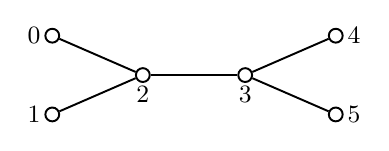
\begin{tikzpicture}[
  scale=0.5,
  line width=0.7pt,
  dot/.style={circle,draw,inner sep=0pt,minimum size=5pt},
  lab/.style={font=\small, inner sep=0pt, outer sep=0pt} % ラベル専用
]
  \coordinate (C2) at (0,0);
  \coordinate (C3) at (2.6,0);
  \coordinate (L0) at (-2.3, 1.0);
  \coordinate (L1) at (-2.3,-1.0);
  \coordinate (R4) at ( 4.9, 1.0);
  \coordinate (R5) at ( 4.9,-1.0);

  \node[dot] (a2) at (C2) {};
  \node[dot] (a3) at (C3) {};
  \node[dot] (a0) at (L0) {};
  \node[dot] (a1) at (L1) {};
  \node[dot] (a4) at (R4) {};
  \node[dot] (a5) at (R5) {};

  \draw (a2)--(a3);
  \draw (a2)--(a0);
  \draw (a2)--(a1);
  \draw (a3)--(a4);
  \draw (a3)--(a5);

%-- labels with explicit coordinates ---
\node[lab,anchor=east]  at (-2.6,  1.00) {$0$};
\node[lab,anchor=east]  at (-2.6, -1.00) {$1$};
\node[lab,anchor=north] at ( 0.00, -0.3) {$2$};
\node[lab,anchor=north] at ( 2.60, -0.3) {$3$};
\node[lab,anchor=west]  at ( 5.2,  1.00) {$4$};
\node[lab,anchor=west]  at ( 5.2, -1.00) {$5$};
\end{tikzpicture}
%\begin{tikzpicture}[
%  scale=0.5,
%  line width=0.7pt,
%  dot/.style={circle,draw,inner sep=0pt,minimum size=5pt},
%  every node/.style={font=\small}
%]
%  %--- backbone coordinates ---
%  \coordinate (C2) at (0,0);
%  \coordinate (C3) at (2.6,0);
%
%  %--- fork endpoints (adjust to taste) ---
%  \coordinate (L0) at (-2.3, 1.0);
%  \coordinate (L1) at (-2.3,-1.0);
%  \coordinate (R4) at ( 4.9, 1.0);
%  \coordinate (R5) at ( 4.9,-1.0);
%
%  %--- nodes (small circles) ---
%  \node[dot] (a2) at (C2) {};
%  \node[dot] (a3) at (C3) {};
%  \node[dot] (a0) at (L0) {};
%  \node[dot] (a1) at (L1) {};
%  \node[dot] (a4) at (R4) {};
%  \node[dot] (a5) at (R5) {};
%
%  %--- edges ---
%  \draw (a2)--(a3);
%  \draw (a2)--(a0);
%  \draw (a2)--(a1);
%  \draw (a3)--(a4);
%  \draw (a3)--(a5);
%
%  %--- labels (outside the circles) ---
%  \node[left=4pt]  at (a0) {$0$};
%  \node[left=4pt]  at (a1) {$1$};
%  \node[below=4pt] at (a2) {$2$};
%  \node[below=4pt] at (a3) {$3$};
%  \node[right=4pt] at (a4) {$4$};
%  \node[right=4pt] at (a5) {$5$};
%
%\end{tikzpicture}
\end{center}
We have $
\pi_4^2=\pi_1,\;
\pi_5=\pi_4^{-1}.
$
For $\pi_4$, the corresponding affine Dynkin automorphism is given by  
$0\mapsto 4,\;
1\mapsto 5,\;
2\mapsto 3,\;
3\mapsto 2,\;
4\mapsto 1,\;
5\mapsto 0.
$
We have
\begin{align*}
\kappa_4&=s_1s_2s_3s_5s_0s_2s_3s_1s_2s_0,\\
\miw{4}&=
s_5s_3s_4s_2s_3s_5s_1s_2s_3s_4.
\end{align*}
As a signed permutation,
$\miw{4}$ is $\bar{5}\bar{4}\bar{3}\bar{2}1$, sending $1$ to $\bar{5}$, $2$ to $\bar{4}$, etc.
We have 
$$
(\miw{4})^2=
\miw{1}=\bar{1}234\bar{5}.
$$
Some of the computations for type \(D_5\) in this paper were carried out
using the SageMath package for extended affine Weyl groups.
\end{example}

% {\color{lightgray}
% For $\sigma\in \Sigma$ and $a\in \ePet$, we denote
% $\sigma(a)=\sigma a\sigma^{-1}$ (\cite[\S 2.4]{ISY}). We have
% \begin{equation}
% \sigma(a)=u_\sigma a u_{\sigma}^{-1},
% \end{equation}
% where $\sigma=t_\sigma u_\sigma$ with $t_\sigma\in X^\lor$ and $u_\sigma \in W_G$ (see \cite[(2.58)]{ISY}).
% In particular, we have
% \begin{equation}
% \pi_i(a)=u_i au_i^{-1}=:u_i(a)
% \end{equation}
% for $a\in \tilde{\Pet}.$
% This is the \emph{left action} of $u_i.$}

% \begin{equation}
% \OGr_{\pi_i}=t_{\varpi_i^\lor}
% \end{equation}


\subsection{Some properties of $\miw{i}$}
\label{sec:Seidel}
% \begin{lem}
% \label{lem:comin}
% For $i\in I$ we have
% \begin{equation}
% i\in I^s\Longleftrightarrow
% \langle \beta ,\piv_i\rangle \in \{-1,0,1\}\quad 
% \text{for all $\beta\in Q$.}
% \end{equation}
% \end{lem}

% {\color{lightgray}
% The following fact holds for arbitarary $i\in I.$
% \begin{prop} For any $i\in I$, we have
%     \begin{equation}
% \inv(w_{i}^{\min}) = \{ \alpha \in \Phi^{+} \mid \pair{\varpi_{i}^{\vee}}{\alpha} > 0\}
% \label{eq:Inv min}
%     \end{equation}
%     for arbitrary $i \in I$. 
% \end{prop}
% \begin{proof}
% Since
%     \ike{$w\varpi_{i}^{\vee} $ is $wt_{\varpi_{i}^{\vee}}$, isn't it?}\kouno{$w\varpi_{i}^{\vee}$ is correct. It is the (usual) action of $W$ on $P^{\vee}$.}
%     \ike{OK thanks. We will make this remark as a lemma.}
%     $w_{i}^{\min}$ is the shortest element of $\{w \in W \mid w(\varpi_{i}^{\vee}) \in -P^{\vee, +}\} = w_{\circ}W_{P_i}$, [Macdonald, (2.4.4)] implies \eqref{eq:Inv min}.
% \end{proof}
% }

% \begin{remark}
%     (cf.\ Naito's pdf) 
    

%     By considering the case $J = I \setminus \{i\}$ for $i \in I^{s}$, we obtain \eqref{eq:long_rep_inv}.
% \end{remark}



Let $R^{+}$ (resp. $ R^-$) be the set of all positive (resp. negative) roots.
For $w \in W$, set 
\begin{equation*}
    \inv(w) := \{\alpha \in R^{+} \mid w(\alpha) \in R^{-} \}. 
\end{equation*}
Note that 
\begin{equation}
    \Des(w) = \{ k \in I \mid \alpha_{k} \in \inv(w)\}. 
    \label{eq:Des roots}
\end{equation}
For $u, v \in W$, it is straightforward to see  
\begin{equation}
    \inv(vw) = (\inv(w) \setminus (-w^{-1}\inv(v))) \sqcup ((w^{-1}\inv(v)) \setminus \inv(w)).
    \label{eq:inv wv}
\end{equation}
 %\kouno{Switching $v$ and $w$ (i.e., use $vw$ instead of $wv$ may make this paper easier to read.}

\begin{lem}For $i \in I^{s}$, we have 
\begin{equation} \label{eq:long_rep_inv}
    \inv(\miw{i}) = \{ \alpha \in R \mid \pair{\varpi_{i}^{\vee}}{\alpha} = 1 \}.  
\end{equation}
\end{lem}
\begin{proof}
For any $i\in I$, we have
    \begin{equation}
\inv(\miw{i}) = \{ \alpha \in R^{+} \mid \pair{\varpi_{i}^{\vee}}{\alpha} > 0\}.
\label{eq:Inv min}
    \end{equation}
    Indeed, 
    $\miw{i}$ is the shortest element in $
    % \{w \in W \mid w(\varpi_{i}^{\vee}) \in -P^{\vee, +}\} =
w_{\circ}W_{P_i}$, therefore \eqref{eq:Inv min} holds by  \cite[(2.4.4)]{Mac}.
Then \eqref{eq:long_rep_inv} holds by \eqref{eq:cominuscule}. 
% {\color{lightgray}
% This follows from Lemma \ref{}, \eqref{}
% , and \eqref{}. }
\end{proof}
\begin{remark}
For $i\in I^s$,
the set \eqref{eq:long_rep_inv} is known to equal to $R_{P_i}^{+},$ the positive part of the root system of $P_i.$
\end{remark}
\section{Proof of the Seidel product theorem }\label{sec:proof}

The following
is a key lemma for the proof of Theorem \ref{thm:main}. 
\begin{lem}\label{lem:key key} For $w\in W$ and $i\in I^s$, we have
\begin{equation}
\gamma_{\miw{i} w}=\gamma_w-w^{-1}(\piv_i).\label{eq:key}
\end{equation}
\end{lem}
% \ike{Dec 29. I made SageMath script to check this equality. gamma-w.ipynb}
\begin{proof}
By applying \eqref{eq:inv wv} with $w=\miw{i}$, we have
% \textcolor{gray}{(, and $\Delta$ the set of all simple roots.)}
% {\color{blue}
 \begin{align*}
 \mathrm{Inv}(\miw{i}w)
 &=\left(\Inv(w)\setminus
 (-w^{-1}\Inv(\miw{i}))\right)
 \sqcup
(w^{-1}\Inv(\miw{i})\setminus\Inv(w) ).
%   \\
%  &=\Inv(v)\setminus \{\}
%  \sqcup
% \{\}
%  \setminus\Inv(v))
 \end{align*}
 By  \eqref{eq:long_rep_inv}
 % \kouno{Jan.~7: \eqref{eq:long_rep_inv}?}\ike{Jan 8. fixed},
 we have
 $$
\pm w^{-1}\Inv(\miw{i})=\{
\alpha\in R\mid \pair{\piv_i}{w(\alpha)}=\pm 1\}.
$$
% By applying \eqref{}
% with $w=\miw{i}$, 
% $\Des(w_{i}^{\min}v)$ is 
% \begin{align}
%         % &= 
%         % \{k\in I\mid \alpha_k\in \mathrm{Inv}(\miw{i}v)\}\quad \text{by \eqref{eq:Des roots}}\\
%         % % &=\{k\in I\mid \pair{\varpi_{i}^{\vee}}{v(\alpha_{k})}\}\\
%         &\{k \mid
%         \pair{\varpi_{i}^{\vee}}{v(\alpha_{k})} = -1\}  \\ &\{k \mid \pair{\varpi_{i}^{\vee}}{v(\alpha_{k})} = 1\} \setminus \Des(v). 
%\end{align}
Therefore we have
\begin{align}
\Des(\miw{i}w)
% &=\{
% k\in I\mid
% \alpha_k\in \Inv(\miw{i}v)\}
% \\
&=I_1\sqcup I_2,\nonumber\\
I_1&=\{
j\in I\mid \alpha_j\in \Inv(w) \;\text{and}\;
\pair{\piv_i}{w(\alpha_j)}\ne -1\}\nonumber\\
&=\Des(w)
\setminus\{j\in I\mid 
\pair{\piv_i}{w(\alpha_j)}= -1\}\nonumber\\
&=\Des(w)\setminus\{j\in \Des(w)\mid 
\pair{\piv_i}{w(\alpha_j)}= -1\},\label{eq:Des minus}
\\
I_2&=
\{j\in I\mid \pair{\piv_i}{w(\alpha_j)}=1\;\text{and} \;\alpha_j\notin \Inv(w)\}\nonumber\\
&
\label{eq:I2 last}=\{j\in I\mid \pair{\piv_i}{w(\alpha_j)}=1\},
% &=(\Des(v)\setminus\{j\in I\mid \pair{\piv_i}{v(\alpha_j)}\ne -1\})\\
% &\sqcup(\{j\in I\mid \pair{\piv_i}{v(\alpha_j)}= 1\}
% \setminus \Des(v))\\
% &=(\Des(v)\setminus\{j\in I\mid \pair{\piv_i}{v(\alpha_j)}\ne -1\})\\
% &\sqcup(\{j\in I\mid \pair{\piv_i}{v(\alpha_j)}=1\}
\end{align}
where \eqref{eq:Des minus}
 and \eqref{eq:I2 last} holds since
$\pair{\piv_i}{w(\alpha_j)}=1$ (resp. $-1$) implies that $w(\alpha_j)\in R^{+}$ (resp. $R^{-}$).
% \begin{align}
%         % &= 
%         % \{j\in I\mid \alpha_j\in \mathrm{Inv}(\miw{i}v)\}\quad \text{by \eqref{eq:Des roots}}\\
%         % % &=\{j\in I\mid \pair{\varpi_{i}^{\vee}}{v(\alpha_{j})}\}\\
%         &\Des(v) \setminus \{j \mid \pair{\varpi_{i}^{\vee}}{v(\alpha_{j})} = -1\}  \\ &\{j \mid \pair{\varpi_{i}^{\vee}}{v(\alpha_{j})} = 1\} \setminus \Des(v). 
% \end{align}
% Observe that 
% \begin{equation}
%     \{j \in I \mid \pair{\varpi_{i}^{\vee}}{v(\alpha_{j})} = -1\} \subset \Des(v)
% \end{equation}
% and 
% \begin{equation}
%     \Des(v) \cap \{j \in I \mid \pair{\varpi_{i}^{\vee}}{v(\alpha_{j})} = 1\} = \emptyset. 
% \end{equation}
% Also, note that 
% \begin{align}
%     v^{-1}(\varpi_{i}^{\vee}) = \sum_{j \in I} \pair{v^{-1}(\varpi_{i}^{\vee})}{\alpha_{j}} \varpi_{j}^{\vee}
% \end{align}
% and that $\pair{v^{-1}(\varpi_{i}^{\vee})}{\alpha_{j}} \in \{0, \pm 1\}$ since $i \in I^{s}$. 
Therefore, we obtain 
\begin{align*}
\gamma_{\miw{i}w} 
    &=
    -\left(\sum_{j\in I_1}
    \piv_j+
    \sum_{j\in I_2}
    \piv_j\right)
\\&=    - \left( \left( \sum_{j \in \Des(w)} \piv_j - \sum_{\substack{j \in \Des(w) \\ \pair{\piv_{i}}{w(\alpha_{j})}=-1}} \piv_j \right) + \sum_{\substack{j \in I \\ \pair{\piv_i}{w(\alpha_{j})}=1}} \piv_j \right) \\&=    - \left( \left( \sum_{j \in \Des(w)} \piv_j - \sum_{\substack{j \in I \\ \pair{\piv_{i}}{w(\alpha_{j})}=-1}} \piv_j \right) + \sum_{\substack{j \in I \\ \pair{\piv_i}{w(\alpha_{j})}=1}} \piv_j \right)\\ 
\\&=    - \left( \left( \sum_{j \in \Des(w)} \varpi_{j}^{\vee} - \sum_{\substack{j \in I \\ \pair{w^{-1}(\piv_{i})}{\alpha_{j}}=-1}} \varpi_{j}^{\vee} \right) + \sum_{\substack{j \in I \\ \pair{w^{-1}(\piv_i)}{\alpha_{j}}=1}} \piv_j \right)\\
&=
\gamma_w
-\sum_{j\in I}
\pair{w^{-1}(\piv_i)}{\alpha_j}\piv_j\quad \text{(by \eqref{eq:cominuscule})} 
\\
    &= \gamma_{w} - w^{-1}(\piv_i), 
\end{align*}
where in the third equality we have used the fact that  
$\pair{\piv_i}{w(\alpha_j)}=-1$ implies $j\in\Des(w)$
again. \end{proof}

\begin{example}\label{ex:D5-2} In type $D_5$, 
we consider $w=s_{2}s_4s_3s_5s_3s_1s_2.$ Then,  $\Des(w)=\{2,5\}$ and $\Des(\miw{4}w)=\{1,3\}$. We have 
$w^{-1}(\piv_4)=
\piv_1-\piv_2+\piv_3-\piv_5.$
\end{example}


\begin{lem}
\label{lem:key}
Let $i$ be any special node, and $w\in W.$ We have
\begin{equation*}
\pi_i^{-1}wt_{\gamma_w}=
\miw{i} wt_{\gamma_{\miw{i} w}}.
\end{equation*}
\end{lem}
% \ike{Dec 28. Maybe we should compare $vt_{\gamma_v}$ and
% $\miw{i} v$.}
\begin{proof}From \eqref{eq:pi inverse}, we have
\begin{align*}
\pi_i^{-1}w
t_{\gamma_w}=
\miw{i} t_{-\piv_i}w
t_{\gamma_w}
=\miw{i}
wt_{-w^{-1}(\piv_i)}t_{\gamma_w}.
\end{align*}
Thus the lemma follows from Lemma \ref{lem:key key}.
\end{proof}



% For $x\in \Wexgr$, and $\sigma\in \Sigma$, we have {\color{magenta}from \eqref{eq:pi on ell}}
% \kouno{This is already mentioned in Lemma~\ref{lem:Sigma acts on L}.}
% \begin{equation}
% \label{eq:sigma acts on ell}
% {u_\sigma}*\OGr_x=\OGr_{\sigma}^{-1}\OGr_{\sigma x}.
% \end{equation}
Let  
$x\in \Wexgr.$ Then 
 from \eqref{eq:pi on ell} and \eqref{eq:pi inverse} we have
\begin{equation}
\label{eq:miw i ell}
\miw{i}*\OGr_x=\OGr_{\pi_i^{-1}}^{-1}\OGr_{\pi_i^{-1}x}.
\end{equation}
 
\begin{proof}[Proof of Theorem \ref{thm:main}] We compute:
% \kouno{Third equality: $t_{\textcolor{red}{\gamma_{v_{i}w}}}$ instead of $t_{v_{i}w}$.}
\begin{align*}
\bO^{\miw{i}}(
\miw{i}*\bO^{w})&=
\frac{\OGr_{\pi_i^{-1}}}{\OGr_{t_{-\piv_i}}}
\miw{i}*\left(
\frac{\OGr_{wt_{\gamma_w}}}{\OGr_{t_{\gamma_w}}}
\right)\quad \text{(by \eqref{eq:Ovi})}\\
&=\frac{\OGr_{\pi_i^{-1}}}{\OGr_{t_{-\piv_i}}}
\frac{(\OGr_{\pi_i^{-1}})^{-1}\OGr_{\pi_i^{-1}wt_{\gamma_w}}}{\OGr_{t_{\gamma_w}}}\quad\text{(by \eqref{eq:miw i ell} and Lemma \ref{lem:W invariance of sigma})}\\
&=\frac{1}{\OGr_{t_{-\piv_i}}}
\frac{\OGr_{\miw{i}wt_{\gamma_{\miw{i}w}}}}{\OGr_{t_{\gamma_w}}}\quad\text{(by Lemma \ref{lem:key})}\\
% &=\frac{\OGr_{t_{\gamma_{\miw{i}w}}}}{\OGr_{t_{-\piv_i}}\OGr_{t_{\gamma_w}}}
% \frac{\OGr_{\miw{i}wt_{\miw{i}w}}}{\OGr_{t_{\gamma_{\miw{i}w}}}}\\
&=
\frac{\OGr_{t_{\gamma_{\miw{i}w}}}}{\OGr_{t_{-\piv_i}}\OGr_{t_{\gamma_w}}}
\bO^{\miw{i}w}\\
&=
\frac{\OGr_{t_{\gamma_w-w^{-1}(\piv_i)}}}{\OGr_{t_{-\piv_i}}\OGr_{t_{\gamma_w}}}
\bO^{\miw{i}w}\quad\text{(by Lemma \ref{lem:key key})}.
\end{align*}
% \ike{Dec 30. Think about $\piv_i-w^{-1}(\piv_i)$.}
% \kouno{Jan.~7: We have $\piv_i-w^{-1}(\piv_i) \in 
% Q^{\vee, +}$. $w^{-1}(\piv_i)$ is a weight of the irreducible highest weight representation of $G^{\vee}$ of highest weight $\piv_{i}$.}
% \ike{Jan 8. Thanks.}
Note that $\piv_i-w^{-1}(\piv_i)$ belongs to the nonnegative integer span of the simple coroots.
Then, by applying $K$-Peterson map, 
% \kouno{Jan.~8: Since $\piv_i-w^{-1}(\piv_i)$ is not anti-dominant, we cannot consider $\ell_{t_{\piv_i-w^{-1}(\piv_i)}}$. We have to apply $K$-Peterson map to $\dfrac{\OGr_{t_{\gamma_w-w^{-1}(\piv_i)}}}{\OGr_{t_{-\piv_i}}\OGr_{t_{\gamma_w}}}
%\bO^{\miw{i}w}$.}, 
we obtain the theorem.
\end{proof}
\subsection{Proof of Corollary \ref{cor:P}}

Let $P$ be an arbitrary standard parabolic subgroup of $G$, and let
$\pi \colon G/B \to G/P$
% \kouno{Is there no risk of confusion with $\pi_{i} \in \Sigma$?}
% \ike{I think no.}
% \kouno{I see.}
be the natural projection. We recall a
pushforward result, due to Kato (\cite{Kato2}).

Denote by $W_P \subset W$ the Weyl group of $P$.
Recall that, for $w\in W$,  $\minrep{w}$ denote the unique minimal-length
representative of the coset $wW_P$. 
% Let $Q_P^\lor = \bigoplus_{i \in I_P} \mathbb{Z}\alpha_i^\lor \subset Q^\lor$
% be the coroot lattice of $P$.
Let $Q^\lor_{\ge 0}:=\sum_{j\in I}\Z_{\ge 0}\alpha_j^\lor$.
\begin{prop}[Kato \cite{Kato2}, Theorem~2.19]\label{prop:push}
There exists a surjective homomorphism of $R(T)$-algebras
\begin{equation*}
\pi_* \colon
QK_T(G/B)
\longrightarrow
QK_T(G/P)
\end{equation*}
sending $\CO^w$ to $\COP^{\minrep{w}}$ for $w \in W$, and $Q^\beta$ to
$Q^{\minrep{\beta}}$ for 
$\beta\in Q^\lor_{\ge 0}.$
\end{prop}

We use the following standard lemma (see, e.g., \cite[Chapter~2]{BB}).
\begin{lem}\label{lem:std}
Let $w \in W^P$ and $i \in I$. If $s_i w > w$ and
$s_i w \notin W^P$, then there exists $j \in I_P$
such that $s_i w = w s_j$.
% \kouno{Do we need a citation (for example, Bjorner--Brenti)?}
\end{lem}
% \begin{proof} It is well known that the map
% $\minrep{\cdot}: W\rightarrow W^P$ is order preserving.
% Now from this fact, we have
% $w=\minrep{w}\le \minrep{s_iw},$
% and therefore $\ell(w)\le\ell(\minrep{s_iw}).$
% Since $s_iw\notin W^P$, we have
% $\minrep{s_iw}<s_i w,$ and hence $\ell(\minrep{s_i w})\le \ell(s_iw)-1=\ell(w).$
% Thus we have $\ell(\minrep{s_i w})
% =\ell(w).$ This equality implies $\minrep{s_iw}=w$ because $w\le \minrep{s_iw}.$ Hence, $s_iw W_P=wW_P$, so there exist $u\in W_P,$ such that $ s_iw=w u$, By the length consideration, we must have $\ell(u)=1$, and therefore $u=s_j$ for some $j\in I_P.$
% \end{proof}

The following result should be known to experts; we include a proof for completeness.

\begin{prop}\label{prop:pi W}
The pushforward 
$\pi_*: QK_T(G/B)\rightarrow QK_T(G/P)$ commutes with the left $W$-action. 
\end{prop}
\begin{proof}
According to \cite[Proposition 8.3 (b)]{MNS}, 
the left action of $W$ on $QK_T(G/P)$ for general parabolic subgroup $P$ is given for $w\in W^P$ and $i\in I$, by 
\begin{equation}
s_i^L \COP^{w}=\begin{cases}
e^{\alpha_i}\COP^{w}+(1-e^{\alpha_i})\COP^{{s_iw}} & \text{if $s_i w<w,$}\\
\COP^{w}& \text{otherwise.}
\end{cases}
\label{eq:def star on CO}
\end{equation}
 Note that this holds for $P=B$ too.

Since the left action of $W$ is a $\mathbb{Z}[Q]$-linear ring automorphism of $QK_T(G/B)$ (\cite[\S 8.3]{MNS}), it suffices to prove 
\begin{equation}
\pi_*(s_i^L\CO^w)=s_i^L\COP^{\minrep{w}}
\quad\text{for all $w\in W$ and $i\in I.$}
\label{eq:pi_commutes_with_W}
\end{equation}
We note that the following holds for $w\in W$ and $i\in I$:
\begin{equation}
s_i\minrep{w}\in W^P
\Longleftrightarrow
s_i\minrep{w}
=\minrep{s_iw}.
\label{eq:minrep}
\end{equation}


{\bf Case 1.} First we consider the case when  $\minrep{s_i w}
=\minrep{w}$ holds. Then 
it is easy from the definition of $\pi_*$ and \eqref{eq:def star on CO} to see that \begin{equation}
    \pi_*(s_i^L\CO^w)=\COP^{\minrep{w}}.\label{eq:pi_O} 
 \end{equation}
 Thus, in order to show \eqref{eq:pi_commutes_with_W}, it suffices to show that 
\begin{equation}
s_i^L\COP^{\minrep{w}}=\COP^{\minrep{w}}.
\label{eq:si inv}\end{equation}
If $s_i\minrep{w}>\minrep{w},$
then \eqref{eq:si inv} holds from \eqref{eq:def star on CO}.
% \kouno{Is this really from definition? \eqref{eq:def star on CO}?} 
% \ike{From \eqref{eq:def star on CO}.}
Now suppose $s_i\minrep{w}<\minrep{w}.$
 Then we have $s_i\minrep{w}\in W^P$ (well known), and so $s_i\minrep{w}
=\minrep{s_iw}$ by \eqref{eq:minrep}. Then it is easy to see 
\eqref{eq:si inv} holds.
% Then \begin{align*}
%      s_i^L
%      \COP^{\minrep{w}}&=e^{\alpha_i}\COP^{\minrep{w}}+(1-e^{\alpha_i})\COP^{s_i\minrep{w}}\\
%      &=e^{\alpha_i}\COP^{\minrep{w}}+(1-e^{\alpha_i})\COP^{\minrep{s_iw}} \\
%      &=e^{\alpha_i}\COP^{\minrep{w}}+(1-e^{\alpha_i})\COP^{\minrep{w}}=\COP^{\minrep{w}}.
%  \end{align*}
 % In fact, 
% if
% $s_iw <w$, we have
% \begin{align*}\pi_*(s_i^L \CO^w)&= \pi_*\left(e^{\alpha_i}\CO^w+(1-e^{\alpha_i})\CO^{{s_i w}})\right)\\
% &=e^{\alpha_i}\COP^{\minrep{w}}+(1-e^{\alpha_i})\COP^{\minrep{s_i w}})
% \\
% &=e^{\alpha_i}\COP^{\minrep{w}}+(1-e^{\alpha_i})\COP^{\minrep{ w}}=\COP^{\minrep{w}}.
% \end{align*}
% If $s_iw>w$ the claim holds obviously.

% Now note that we have
% $s_i \minrep{w}<\minrep{w},$ since
% $s_i \minrep{w}W_P=
% s_i wW_P.$ Hence we have
% \begin{align*}
%     s_i^L \COP^{\minrep{w}}&=e^{\alpha_i}\COP^{\minrep{w}}+(1-e^{\alpha_i})\COP^{s_i\minrep{w}}\\
%     &=e^{\alpha_i}\COP^{\minrep{w}}+(1-e^{\alpha_i})\COP^{\minrep{w}}=\COP^{\minrep{w}}.
% \end{align*}


{\bf Case 2.} Next, we consider the case when 
$\minrep{s_iw}\ne \minrep{w}.$
We claim  
\begin{equation}
\label{eq:si minrep}
s_i\minrep{w}\in W^P.
\end{equation}
Indeed, if 
$s_i\minrep{w}< \minrep{w}$, then 
\eqref{eq:si minrep} holds.
Now assume $s_i\minrep{w}> \minrep{w}$ and $s_i\minrep{w}\notin W^P$. Then we have 
$s_i\minrep{w}W_P=\minrep{w}W_P$ by Lemma \ref{lem:std}, which means $\minrep{s_iw}=\minrep{w}.$ This contradicts the assumption, so \eqref{eq:si minrep} holds.




Now assume $s_iw<w.$
Then it ais straightforward to
see \eqref{eq:pi_commutes_with_W} holds.
% one sees that $\minrep{s_i w}=s_i\minrep{w}<\minrep{w}$. Therefore
% \begin{align*}
% \pi_*(s_i^L\CO^w)&=
% \pi_*(e^{\alpha_i}\CO^w
% +(1-e^{\alpha_i})
% \CO^{s_iw})\\
% &=e^{\alpha_i}\COP^{\minrep{w}}
% +(1-e^{\alpha_i})
% \COP^{\minrep{s_iw}}\\
% &=e^{\alpha_i}\COP^{\minrep{w}}
% +(1-e^{\alpha_i})
% \COP^{s_i\minrep{w}}\\&=
% s_i^L \COP^{\minrep{w}}.
% \end{align*}

Finally, we consider the case $s_iw>w$.
We have $\minrep{s_iw}\ge \minrep{w}$.
We know that $s_i\minrep{w}=\minrep{s_iw}$ holds since  \eqref{eq:si minrep} holds. Therefore, we have $s_i\minrep{w}>\minrep{w}.$
Then we have
$s_i^L\CO^w=\CO^w$ and $s_i^L\COP^{\minrep{w}}=\COP^{\minrep{w}}$, and 
\eqref{eq:pi_commutes_with_W} is fulfilled.
\end{proof}



\begin{proof}[Proof of Corollary \ref{cor:P}]
The corollary is 
obtained from Theorem \ref{thm:main} by Proposition \ref{prop:push} and Proposition \ref{prop:pi W}.
\end{proof}
 \appendix
\section{Extended $K$-Peterson algebra}\label{sec:ePetA}
The purpose of this section is to give a brief explanation of the construction in \cite[\S 2]{ISY}. 
%We also discuss the $\Sigma$-grading of $\ePet.$
\subsection{Extended level-zero $K$-nil-Hecke algebra $\hat{\mathbb{K}}_\af$}
\label{sec:K_nil}
Consider an action of $\hat{W}_\af$ on $R(T^\ad)=\Z[Q]$ given 
by 
\begin{equation*}
(t_\gamma w)e^\beta=e^{w(\beta)}\quad (\gamma\in P^\lor,\;w\in W,\; \beta\in Q),
\end{equation*}
where $w(\beta)$ denotes the natural action of $w$ on $\beta$.
This is called the \emph{level zero action}.
In particular $s_0$ acts on $\Z[Q]$ by $s_{\theta}$.
The action extends to the field $\F:=\mathrm{Frac}\,R(T^\ad)$ of fractions of $R(T^\ad)$.
The twisted group ring 
$\F[\hat{W}_\af]$ is
$\F\otimes_\Z \Z[\hat{W}_\af]$ as a left $\F$-module, 
equipped with the product
$$
(f\otimes w)(g\otimes v)=fw(g)\otimes wv \quad(f,g\in \F,\;
w,v\in W).
$$
We simply denote $f\otimes w$ by $fw.$
Let $\theta\in R$ be the highest root.
For $i\in I$, 
the corresponding simple root is denoted by  $\alpha_i$, here we understood $\alpha_0$ to be $-\theta$. 
For $i\in I_\af$, define
\begin{equation}
D_i=(1-e^{\alpha_i})^{-1}({s_i-1})+1
\in \F[W_\af].
\end{equation}
The elements $D_i\;(i\in I_\af)$ satisfy the braid relation and
$
D_i^2=D_i.
$ For $w\in W_\af$, take an reduced expression  $w=s_{i_1}\cdots s_{i_r}$. Then $D_w=D_{i_1}\cdots D_{i_r}$ is defined.

For $\sigma w\in \hat{W}_\af\;(\sigma \in\Sigma, \, w\in W_\af)$, define
$D_{\sigma w}=\sigma D_w.$ The extended level zero $K$- nil-Hecke algebra 
$\hat{\mathbb{K}}_\af$
is the left $R(T^\ad)$-module generated by 
$D_x\;(x\in \hat{W}_\af).$ This is indeed a ring, but the ``scalars'' $R(T^\ad)$ 
are not central. 
% Note that $\hat{W}_\af$ is contained in the twisted group ring.  
% We define \begin{equation*}
%     \ePet=Z_{\hat{\mathbb{K}}_\af}(R(T^\ad))=\{
%     a\in \hat{\mathbb{K}}_\af\mid a f=fa\quad\text{for all $f\in R(T^\ad)$}\},
% \end{equation*}
Let $\ePet$ be the centralizer subalgebra of $R(T^\ad)$ in $\hat{\mathbb{K}}_\af.$
Note that $t_\gamma\;(\gamma\in P^\lor)$
is an element of $\ePet.$

% \subsection{Star action of $\hat{\mathbb{K}}_\af$ on $\ePet$}
% \label{sec:star action}
% There is a fundamental action of $\hat{\mathbb{K}}_\af$ on the Peterson algebra $\ePet.$ The idea goes back to Peterson in homology setting \cite{Pet}. 
% \begin{prop}[\cite{ISY}]
% $\ePet$ has a left 
% $\hat{\mathbb{K}}_\af$-module structure
% such that for $f\in R(T^\ad), w\in {W}_\af, t_{\gamma}\;(\gamma\in P^\lor)$,
% \begin{align}
% f* a&=f a,\\
% w*a&=waw^{-1},\label{eq:act conj}\\
% t_\gamma* a&=
% t_\gamma a
% \end{align}
% for all $a\in \ePet.$
% \end{prop}
% This action is called the \emph{star action} in \cite{ISY}. 
% % \begin{remark}
% % The action of $w\in W$ given by \eqref{eq:act conj} corresponds to the left action of $w$ on $K_*^{T^\ad}(\Gr_{G^\ad}).$ 
% % \end{remark}

\subsection{Schubert basis of $\ePet$}
There is a fundamental action of $\hat{\mathbb{K}}_\af$ on the Peterson algebra $\ePet.$
By using the star action, we can construct the Schubert basis of $\ePet.$

\begin{defn}\label{defn:l-basis}
%\kouno{Do we use ``remark style" for the definition?}
For $x\in \hat{W}_\af^0,$ define
$\OGr_x:=D_x*1\in \ePet.$
\end{defn}
% \begin{example}
% For $\sigma\in \Sigma$,
% we write $\sigma=t_{\gamma_\sigma}u_\sigma$ with $\gamma_\sigma\in P^\lor,\; u_\sigma\in W.$ Then 
% \begin{equation*}
% \ell_\sigma
% =D_\sigma*1=
% \sigma *1=t_{\gamma_\sigma} u_\sigma 1 u_\sigma^{-1}=t_{\gamma_\sigma}.
% \end{equation*} 
% For $\sigma,\sigma'\in \Sigma$, since
% $\sigma \sigma'
% % =
% % t_{\gamma_\sigma} u_\sigma t_{\gamma_{\sigma'}}u_{\sigma'}=t_{\gamma_\sigma} (u_\sigma t_{\gamma_{\sigma'}}
% % u_\sigma^{-1})
% % u_\sigma u_{\sigma'}
% =t_{\gamma_\sigma}t_{u_\sigma(\gamma_{\sigma'})} u_\sigma u_{\sigma'}$ we have 
% \begin{equation*}
% \OGr_{\sigma\sigma'}=
% t_{\gamma_\sigma}t_{u_\sigma(\gamma_{\sigma'})} =\OGr_{\sigma}
% t_{u_\sigma(\gamma_{\sigma'})}
% =\OGr_{\sigma}
% u_\sigma t_{\gamma_{\sigma'}}
% u_\sigma^{-1}=
% \OGr_{\sigma}
% (u_\sigma*\OGr_{\sigma'}).
% \end{equation*}
% This is \eqref{eq: ell sigma sigma}.
% \end{example}


\begin{prop}[{\cite[Proposition 2.24]{ISY}}]\label{prop:D acts on ell}
Let $i\in I_\af$ and $x\in \hat{W}_\af^0$. Then we have 
\begin{equation*}
D_i*\ell_x=\begin{cases}
    \ell_{s_i x} & \text{if $\ell(s_ix)>\ell(x)$ and $s_i x\in \hat{W}_\af^0$,}\\
    \ell_x &\text{otherwise}.
\end{cases}
\end{equation*}
\end{prop}
\begin{thm}[{\cite[Theorem 2.15]{ISY}}]
We have 
$\ePet=\bigoplus_{x\in \hat{W}_\af^0} R(T^\ad)\ell_x.$
\end{thm}

\begin{remark}Non-extended verion of 
$K$-nil-Hecke algebra 
$\mathbb{K}_\af$, and that of the Peterson algebra $\Pet
$
are defined similarly.
$\Pet$ has an $R(T)$-basis $\{\ell_x\mid x\in W_\af^0\}$ defined similarly, by using only $D_x$ for $x\in W_\af^0.$
\end{remark}

\subsection{Star action of $W_\af$ on Schubert basis elements}
\begin{prop}
For $i\in I_\af$, we have 
\begin{equation}
s_i* a=e^{\alpha_i}a
+(1-e^{\alpha_i})D_i *a
\quad \text{for all $a\in \ePet$}.
\label{eq:left action def}
\end{equation}
In particular, for $x\in \hat{W}_\af^0$ and $i\in I_\af$, we have
\begin{equation}
s_i* \ell_x=\begin{cases}
 e^{\alpha_i}\ell_x
+(1-e^{\alpha_i})\ell_{s_i x}& \text{if $s_ix>x$ and $s_i x\in \hat{W}_\af^0$,} \\
\ell_x & \text{otherwise}.
\end{cases}
\label{eq:left on ell}
\end{equation}
\end{prop}
\begin{proof}
\eqref{eq:left action def} is the definition of $D_i*a$.
\eqref{eq:left on ell} is equivalent to
Proposition \ref{prop:D acts on ell}.
\end{proof}

% \begin{remark}
% Let $\hat{\F}=\mathrm{Frac}\, R(T).$ The field extension $\hat{\F}/\F$ is algebraic and of degree $\# \Sigma.$
% In fact, for any representatives $\{\gamma_j\}\subset P^\lor$ for the coset $P^\lor/Q^\lor,$
% $\{e^{\gamma_j}\}$ is 
% an $\F$-basis of $\hat{\F}.$
% \end{remark}

\subsection{Proof of Proposition \ref{prop:W_commutes}}
\label{ssec:proof_W_commutes}

\begin{lem}[{\cite[Lemma 6.7]{CP}}]\label{lem:CP}
Let $x\in W_\af^0$.
Write 
$x=wt_\beta$ with $w\in W$ and $\beta\in Q^\lor$. 
For $i\in I$, we have 
\begin{equation*}
s_ix>x\;\;\text{and}\;\; s_ix\in W_\af^0
\Longleftrightarrow
s_iw<w.
\end{equation*}
\end{lem}
% \begin{proof} {\color{lightgray}$(\Longrightarrow)$
% Suppose, for contradiction, that $s_i w<w$. It is known that this is equivalent to $w^{-1}(\alpha_i)<0.$
% Since $s_ix=s_i wt_\beta\notin W_\af^0$, there is $j\in I$ such that 
% $\pair{\beta}{\alpha_j}=0$ and $s_i w(\alpha_j)<0$ (see \cite[Lemma 3.3]{LS:Acta}).
% On the other hand, from the assumption $wt_\beta\in W^0_\af$, we obtain  $w(\alpha_j)>0$, again by \cite[Lemma 3.3]{LS:Acta}. Therefore we must have $w(\alpha_j)=\alpha_i$ (see for example \cite[Lemma 4.4.3]{BB}), and hence $w^{-1}(\alpha_i)=\alpha_i.$
% This contradicts the conclusion above that $w^{-1}(\alpha_i)<0.$}
% \end{proof}

\begin{proof}[Proof of Proposition \ref{prop:W_commutes}]
We will show
\begin{equation}
\Phi(s_i *\bO^w)=s_i^L 
\CO^w\quad \text{for $w\in W$ and $i\in I$.}
\label{eq:Phi_commutes_W}
\end{equation}
Recall the formula of $W$-action on $\{\CO^w\mid w\in W\}:$
\begin{equation}
\label{eq:W acts CO}
s_i^L
\CO^w=\begin{cases}
e^{\alpha_i}\CO^w+(1-e^{\alpha_i})\CO^{s_iw} & \text{if $s_i w<w$,}\\
\CO^w & \text{if $s_iw>w$.}
\end{cases}
\end{equation}
Then \eqref{eq:Phi_commutes_W}
is clear from Lemma \ref{lem:CP}, Lemma \ref{lem:W invariance of sigma} and \eqref{eq:left on ell}.
\end{proof}


\section{Examples}\label{sec:exa}
This appendix collects several examples illustrating applications of the results developed in the main text.
\subsection{Type $A_{n-1}$}
In type $A_{n-1}$,
we have $I=\{1,\ldots,n-1\}$.
All elements in $I$ are special and $\Sigma\cong \Z/n\Z.$
For $i\in I^s$,
$\miw{i}$ is the longest  
$i$-Grassmannian permutation $(i+1,i+2,\ldots,n,1,2,\ldots, i)$ in one-line notation.

In type $A_2$, we have
$
\miw{1}=s_2s_1,\; \miw{2}=s_1s_2,
$
and 
\begin{align*}
\bO^{s_1}=\frac{\ell_{\pi_1^{-1}s_0}}{\sigma_1},\quad
\bO^{s_2}=\frac{\ell_{\pi_2^{-1}s_0}}{\sigma_2},\quad
\bO^{s_1s_2}=\frac{\ell_{\pi_2^{-1}}}{\sigma_2},\quad
\bO^{s_2s_1}=\frac{\ell_{\pi_1^{-1}}}{\sigma_1},\quad
\bO^{w_\circ}=\frac{\ell_{s_0}}{\sigma_1\sigma_2},
\end{align*}
and $
Q_1=\dfrac{\sigma_2}{\sigma_1^2},\;
Q_2=\dfrac{\sigma_1}{\sigma_2^2},
$
where by abuse of notation we 
simply denote  $\prod_{j\in I}\sigma_{j}^{-\pair{\alpha_k^\lor}{\alpha_j}}$by $Q_k.$
Let us consider $i=2.$ For example, we have by \eqref{eq:miw i ell},
 \begin{align*}
 \bO^{\miw{2}}\cdot
 (\miw{2}*{\bO^{s_1}})&
=\frac{\ell_{\pi_2^{-1}}}{\sigma_2}
\miw{2}*\left({\frac{\ell_{\pi_1^{-1}s_0}}{\sigma_1}}\right)=\frac{\ell_{\pi_2^{-1}}}{\sigma_2}
{\frac{(\ell_{\pi_2^{-1}})^{-1}\ell_{\pi_2^{-1}\pi_1^{-1}s_0}}{\sigma_1}}\\
&=\frac{\ell_{s_0}}{\sigma_1\sigma_2}
=\bO^{w_\circ},
\end{align*}
% \kouno{Are positions of parenthesis correct? (same for below)}
% \ike{Feb 19. I do not see your concern.... I edited a little anyway.}
% %
% %
% %
% \begin{align*}
% \bO^{\miw{2}}\cdot
% \miw{2}*({\bO^{s_2}})&=\frac{\ell_{\pi_2^{-1}}}{\sigma_2}
% \miw{2}*
% \left({\frac{\ell_{\pi_2^{-1}s_0}}{\sigma_2}}\right)
% =\frac{\ell_{\pi_2^{-1}}}{\sigma_2}
% {\frac{(\ell_{\pi_2^{-1}})^{-1}\ell_{\pi_2^{-1}\pi_2^{-1}s_0}}{\sigma_2}}\\
% &=\frac{\sigma_1}{\sigma_2^2}\frac{\ell_{\pi_1^{-1}s_0}}{\sigma_1}
% =Q_2\bO^{s_1}.
% \end{align*}


The remaining cases (except for $w=e$) are given as follows: 
\begin{align*}
\bO^{\miw{2}}\cdot
(\miw{2}*{\bO^{s_2}})&=Q_2\bO^{s_1},\quad
\bO^{\miw{2}}\cdot(\miw{2}*{\bO^{s_1s_2}})=
Q_2\bO^{s_2s_1},\\
\bO^{\miw{2}}\cdot(\miw{2}*{\bO^{s_2s_1}})&=Q_1Q_2,\quad
\bO^{\miw{2}}\cdot(\miw{2}*{\bO^{w_\circ}})=Q_1Q_2\bO^{s_2}.
\end{align*}


\subsection{Type $C_2$}
In type $C_n$, $I=\{1,2,\ldots,n\}$ and we have $I^s=\{n\},$ and $
\miw{n}=s_n
(s_{n-1}s_n)\cdots (s_2 \cdots s_{n-1}s_n)
(s_1s_2 \cdots s_{n-1}s_n).
$

In type $C_2$, we have 
$\miw{2}=s_2s_1s_2$. We have
\begin{align*}
\bO^{s_1}&=\frac{\ell_{s_2s_1s_0}}{\sigma_1},\quad
\bO^{s_2}=
\frac{\ell_{\pi_2^{-1}s_1s_0}}{\sigma_2},\quad
\bO^{s_1s_2}=
\frac{\ell_{\pi_2^{-1}s_0}}{\sigma_2},\quad
\bO^{s_2s_1}=
\frac{\ell_{s_1s_0}}{\sigma_1},\\
\bO^{s_1s_2s_1}&=
\frac{\ell_{s_0}}{\sigma_1},\quad
\bO^{\miw{2}}=\bO^{s_2s_1s_2}
=\frac{\ell_{\pi_2^{-1}}}{\sigma_2},\quad
\bO^{w_\circ}=
\frac{\ell_{\pi_2^{-1}s_2s_1s_0}}{\sigma_1\sigma_2},
\end{align*}
and 
$
Q_1=\dfrac{\sigma_2^2}{\sigma_1^2},\quad
Q_2=\dfrac{\sigma_1}{\sigma_2^2}.
$ 
The following table lists $\bO^{v_2}\cdot v_2*\bO^w$ for $w\in W$.
% We have
% \begin{align*}
% \bO^{{\miw{2}}}\cdot \miw{2}*{\bO^{s_2s_1s_2}}&
% % =
% % \frac{\ell_{\pi_2^{-1}}}{\sigma_2}\frac{(\ell_{\pi_2^{-1}})^{-1}\ell_{\pi_2^{-1}\pi_2^{-1}}}{\sigma_2}
% =\frac{1}{\sigma_2^2
% }=
% Q_1Q_2^2,\\
% %
% %
% \bO^{\miw{2}}\cdot\miw{2}*{\bO^{w_\circ}}&
% % =\frac{\ell_{\pi_2^{-1}}}{\sigma_2}
% % \frac{(\ell_{\pi_2^{-1}})^{-1}{\ell_{\pi_2^{-1}\pi_2^{-1}s_2s_1s_0}}}{\sigma_1\sigma_2}
% =\frac{1}{\sigma_2^2}\frac{\ell_{s_2s_1s_0}}{\sigma_1}
% =Q_1Q_2^2\bO^{s_1},\\
% %
% %
% %
% \bO^{\miw{2}}\cdot\miw{2}*{\bO^{s_2}}
% &
% % =\frac{\ell_{\pi_2^{-1}}}{\sigma_2}\frac{(\ell_{\pi_2^{-1}})^{-1}\ell_{\pi_2^{-1}\pi_2^{-1}s_1s_0}}{\sigma_2}
% =\frac{\sigma_1}{\sigma_2^2}\frac{\ell_{s_1s_0}}{\sigma_1}
% =Q_2\bO^{s_2s_1},
% \\
% %
% %
% \bO^{\miw{2}}\cdot\miw{2}*{\bO^{s_1}}&
% % =
% %  \frac{\ell_{\pi_2^{-1}}}{\sigma_2}
% %  \frac{\overline{\ell_{s_2s_1s_0}}}{\sigma_1}
%  =
% \frac{{\ell_{\pi_2^{-1}s_2s_1s_0}}}{\sigma_1\sigma_2}
%  =\bO^{w_\circ}, \\
%  %
%  %
% \bO^{\miw{2}}\cdot\miw{2}*{\bO^{s_1s_2}}&
% % =
% %  \frac{\ell_{\pi_2^{-1}}}{\sigma_2}
% % \frac{(\ell_{\pi_2^{-1}})^{-1}{\ell_{s_0}}}{\sigma_2}
% =
%  \frac{\sigma_1}{\sigma_2^2}
%  \frac{\ell_{s_0}}{\sigma_1}=Q_2 \bO^{s_1s_2s_1},\\
%  %
%  %
% \bO^{\miw{2}}\cdot\miw{2}*{\bO^{s_2s_1}}&
% % =
% %  \frac{\ell_{\pi_2^{-1}}}{\sigma_2}
% %  \frac{\overline{\ell_{s_1s_0}}}{\sigma_1}
%  =
%  \frac{1}{\sigma_1}
%  \frac{\ell_{\pi_2^{-1}s_1s_0}}{\sigma_2}=Q_1Q_2 \bO^{s_2}
% ,\\
% %
% %
% \bO^{\miw{2}}\cdot\miw{2}*{\bO^{s_1s_2s_1}}
% &
% % = \frac{\ell_{\pi_2^{-1}}}{\sigma_2}
% % \frac{\overline{\ell_{s_0}}}{\sigma_1}
% =
%  \frac{1}{\sigma_1}
%  \frac{\ell_{\pi_2^{-1}s_0}}{\sigma_2}=Q_1Q_2 \bO^{s_1s_2}.
%  \end{align*}

%  \[
% \renewcommand{\arraystretch}{1.3}
% \begin{array}{rcl}
% \bO^{\miw{2}}\cdot \miw{2}*{\bO^{s_2s_1s_2}}
% &=& Q_1Q_2^2, \\

% \bO^{\miw{2}}\cdot \miw{2}*{\bO^{w_\circ}}
% &=& Q_1Q_2^2\,\bO^{s_1}, \\

% \bO^{\miw{2}}\cdot \miw{2}*{\bO^{s_2}}
% &=& Q_2\,\bO^{s_2s_1}, \\

% \bO^{\miw{2}}\cdot \miw{2}*{\bO^{s_1}}
% &=& \bO^{w_\circ}, \\

% \bO^{\miw{2}}\cdot \miw{2}*{\bO^{s_1s_2}}
% &=& Q_2\,\bO^{s_1s_2s_1}, \\

% \bO^{\miw{2}}\cdot \miw{2}*{\bO^{s_2s_1}}
% &=& Q_1Q_2\,\bO^{s_2}, \\

% \bO^{\miw{2}}\cdot \miw{2}*{\bO^{s_1s_2s_1}}
% &=& Q_1Q_2\,\bO^{s_1s_2}.
% \end{array}
% \]

% \[
% \begin{array}{lcl}
% \bO^{\miw{2}}\cdot \miw{2}*{\bO^{s_2s_1s_2}} &=& Q_1Q_2^2,\\
% \bO^{\miw{2}}\cdot \miw{2}*{\bO^{w_\circ}}   &=& Q_1Q_2^2\,\bO^{s_1},\\
% \bO^{\miw{2}}\cdot \miw{2}*{\bO^{s_2}}       &=& Q_2\,\bO^{s_2s_1},\\
% \end{array}
% \]

% \begin{center}
% \renewcommand{\arraystretch}{1.4}
% \begin{tabular}{c|c|c|c}
% $w$ 
% & $s_2s_1s_2$ 
% & $w_\circ$ 
% & $s_2$ \\ \hline
% $\bO^{\miw{2}}\cdot \miw{2}* \bO^w$
% & $Q_1Q_2^2$
% & $Q_1Q_2^2\,\bO^{s_1}$
% & $Q_2\,\bO^{s_2s_1}$
% \end{tabular}

% \vspace{0.8em}

% \begin{tabular}{c|c|c|c}
% $w$
% & $s_1$
% & $s_1s_2$
% & $s_2s_1$ \\ \hline
% $\bO^{\miw{2}}\cdot \miw{2}* \bO^w$
% & $\bO^{w_\circ}$
% & $Q_2\,\bO^{s_1s_2s_1}$
% & $Q_1Q_2\,\bO^{s_2}$
% \end{tabular}

% \vspace{0.8em}

% \begin{tabular}{c|c}
% $w$ 
% & $s_1s_2s_1$ \\ \hline
% $\bO^{\miw{2}}\cdot \miw{2}* \bO^w$
% & $Q_1Q_2\,\bO^{s_1s_2}$
% \end{tabular}
% \end{center}

% \begin{center}
% \renewcommand{\arraystretch}{1.4}
% \begin{tabular}{c|ccccccc}
% $w$
% & $s_1$
% & $s_2$
% & $s_1s_2$
% & $s_2s_1$
% & $s_1s_2s_1$
% & $s_2s_1s_2$
% & $w_\circ$ \\ \hline
% $\bO^{\miw{2}}\cdot \miw{2}* \bO^w$
% & $\bO^{w_\circ}$
% & $Q_2\,\bO^{s_2s_1}$
% & $Q_2\,\bO^{s_1s_2s_1}$
% & $Q_1Q_2\,\bO^{s_2}$
% & $Q_1Q_2\,\bO^{s_1s_2}$
% & $Q_1Q_2^2$
% & $Q_1Q_2^2\,\bO^{s_1}$
% \end{tabular}
% \end{center}

% \begin{center}
% \renewcommand{\arraystretch}{1.4}

% \begin{tabular}{c|c|c|c|c}
% $w$
% & $s_1$
% & $s_2$
% & $s_1s_2$
% & $s_2s_1$ \\ \hline
% $v_2(\bO^w)$
% & $\bO^{w_\circ}$
% & $Q_2\,\bO^{s_2s_1}$
% & $Q_2\,\bO^{s_1s_2s_1}$
% & $Q_1Q_2\,\bO^{s_2}$
% \end{tabular}

% \vspace{1em}

% \begin{tabular}{c|c|c|c}
% $w$
% & $s_1s_2s_1$
% & $s_2s_1s_2$
% & $w_\circ$ \\ \hline
% $v_2(\bO^w)$
% & $Q_1Q_2\,\bO^{s_1s_2}$
% & $Q_1Q_2^2$
% & $Q_1Q_2^2\,\bO^{s_1}$
% \end{tabular}

% \end{center}

% \begin{center}
% \renewcommand{\arraystretch}{1.4}
% \begin{tabular}{c|ccccccc}
% $w$
% & $s_1$
% & $s_2$
% & $s_1s_2$
% & $s_2s_1$
% & $s_1s_2s_1$
% & $s_2s_1s_2$
% & $w_\circ$ \\ \hline
% $v_2(\bO^w)$
% & $\bO^{w_\circ}$
% & $Q_2\,\bO^{s_2s_1}$
% & $Q_2\,\bO^{s_1s_2s_1}$
% & $Q_1Q_2\,\bO^{s_2}$
% & $Q_1Q_2\,\bO^{s_1s_2}$
% & $Q_1Q_2^2$
% & $Q_1Q_2^2\,\bO^{s_1}$
% \end{tabular}
% \end{center}

\begin{center}
\renewcommand{\arraystretch}{1.4}
\begin{tabular}{c|c|c|c|c|c|c}
$s_1$
& $s_2$
& $s_1s_2$
& $s_2s_1$
& $s_1s_2s_1$
& $s_2s_1s_2$
& $w_\circ$ \\ \hline
$\bO^{w_\circ}$
& $Q_2\,\bO^{s_2s_1}$
& $Q_2\,\bO^{s_1s_2s_1}$
& $Q_1Q_2\,\bO^{s_2}$
& $Q_1Q_2\,\bO^{s_1s_2}$
& $Q_1Q_2^2$
& $Q_1Q_2^2\,\bO^{s_1}$
\end{tabular}
\end{center}


%  \begin{center}
% \renewcommand{\arraystretch}{1.8}
% \begin{tabular}{ccccccc}
% $s_1$
% & $s_2$
% & $s_1s_2$
% & $s_2s_1$
% & $s_1s_2s_1$
% & $s_2s_1s_2$
% & $w_\circ$ \\ \hline

% $\displaystyle 
% \frac{\ell_{\pi_2^{-1}s_2s_1s_0}}{\sigma_1\sigma_2}$
% & $\displaystyle 
% \frac{\sigma_1}{\sigma_2^2}\frac{\ell_{s_1s_0}}{\sigma_1}$
% & $\displaystyle 
% \frac{\sigma_1}{\sigma_2^2}\frac{\ell_{s_0}}{\sigma_1}$
% & $\displaystyle 
% \frac{1}{\sigma_1}\frac{\ell_{\pi_2^{-1}s_1s_0}}{\sigma_2}$
% & $\displaystyle 
% \frac{1}{\sigma_1}\frac{\ell_{\pi_2^{-1}s_0}}{\sigma_2}$
% & $\displaystyle 
% \frac{1}{\sigma_2^2}$
% & $\displaystyle 
% \frac{1}{\sigma_2^2}\frac{\ell_{s_2s_1s_0}}{\sigma_1}$ \\[0.6em]

% $\bO^{w_\circ}$
% & $Q_2\,\bO^{s_2s_1}$
% & $Q_2\,\bO^{s_1s_2s_1}$
% & $Q_1Q_2\,\bO^{s_2}$
% & $Q_1Q_2\,\bO^{s_1s_2}$
% & $Q_1Q_2^2$
% & $Q_1Q_2^2\,\bO^{s_1}$
% \end{tabular}
% \end{center}

% \begin{align*}
% \bO^{{\miw{2}}}\cdot \miw{2}*{\bO^{s_2s_1s_2}}&
% =\frac{1}{\sigma_2^2
% }=
% Q_1Q_2^2,\\
% \bO^{\miw{2}}\cdot\miw{2}*{\bO^{w_\circ}}&
% =\frac{1}{\sigma_2^2}\frac{\ell_{s_2s_1s_0}}{\sigma_1}
% =Q_1Q_2^2\bO^{s_1},\\
% \bO^{\miw{2}}\cdot\miw{2}*{\bO^{s_2}}
% &
% =\frac{\sigma_1}{\sigma_2^2}\frac{\ell_{s_1s_0}}{\sigma_1}
% =Q_2\bO^{s_2s_1},
% \\
% \bO^{\miw{2}}\cdot\miw{2}*{\bO^{s_1}}&
%  =
% \frac{{\ell_{\pi_2^{-1}s_2s_1s_0}}}{\sigma_1\sigma_2}
%  =\bO^{w_\circ}, \\
% \bO^{\miw{2}}\cdot\miw{2}*{\bO^{s_1s_2}}&
% =
%  \frac{\sigma_1}{\sigma_2^2}
%  \frac{\ell_{s_0}}{\sigma_1}=Q_2 \bO^{s_1s_2s_1},\\
% \bO^{\miw{2}}\cdot\miw{2}*{\bO^{s_2s_1}}&
%  =
%  \frac{1}{\sigma_1}
% \frac{\ell_{\pi_2^{-1}s_1s_0}}{\sigma_2}=Q_1Q_2 \bO^{s_2}
% ,\\
% \bO^{\miw{2}}\cdot\miw{2}*{\bO^{s_1s_2s_1}}
% &=
%  \frac{1}{\sigma_1}
%  \frac{\ell_{\pi_2^{-1}s_0}}{\sigma_2}=Q_1Q_2 \bO^{s_1s_2}.
%  \end{align*}



\subsection{Type $D_5$}
Consider type $D_5$ and $i=4.$
Let $w\in W$ be the element in Example \ref{ex:D5-2}. We have
$
\piv_4-w^{-1}\piv_4=
\alpha_2^\lor+\alpha_3^\lor+\alpha_4^\lor+\alpha_5^\lor.$
Therefore
we have
$$
\CO^{\miw{4}}
\cdot \miw{4}^L\CO^{w}
=Q_2Q_3Q_4Q_5
\CO^{\miw{4} w}.
$$

%\input{A2.tex}



% \section{Left $W$-action}

% \subsection{Automorphism $\alpha$ of $QK_T(G/B)$}
% For $w\in W,$ $X_w
% $ denotes the Zariski clocure of $B\dot{w}/B\cong \C^{\ell(w)}.$




% \begin{prop}
% There is an automorphism $\alpha$  of 
% $QK_T(G/B)$ satisfying 
% \begin{equation}
%     e^\lambda \mathscr{O}_{X_{ww_\circ} }\mapsto e^{w_\circ \lambda }\CO^{w_\circ ww_\circ }.
% \end{equation}    
% \end{prop}

% $\dot{w_\circ}$

% \subsection{Bar automorphism}
% Let $\overline{()}$ be the ring automorphism of $QK_T(G/B)$ given by 
% \begin{equation}
% \overline{e^\lambda}=e^{-\lambda},\quad
% \overline{\CO^{w}}
% ={\CO^w}
% \quad \text{for $\lambda\in P^\lor$ and $w\in W$}.
% \end{equation}

% \begin{equation}
% \Phi'(\bO^w)
% \mapsto \mathscr{O}_{X_{ww_\circ}}
% \end{equation}
% \subsection{Comparizon }
% \begin{equation}
% \Phi=
% \end{equation}
% \begin{remark}
% In \cite{Kato}, 
% $\mathscr{O}_{X_{ww_\circ}} $ is
% denoted by ``$\mathscr{O}^w$'' which is not equal to
% our $\CO^w.$
% \end{remark}


% \begin{lem}
% $\miw{i}(\CO^{\miw{i}})
% $ is invariant by 
% the bar automorphism.
% \end{lem}

% \subsection{Precise identification of Maps}
% \begin{prop}
% $\Phi=$  
% \end{prop}

% \begin{lem}
% Let $x=wt_\gamma\in W_\af^0.$ We have (\cite[Lemma 6.7]{CP}, $\ell(wt_\lambda)$ see \cite{LS})
% \begin{equation}
% s_i x\in W_\af^0\;\text{and $s_i x>x$}
% \Longleftrightarrow
% s_i w<w.
% \end{equation}
% \end{lem}

% \begin{prop}
% $\Phi $ commutes with the left $W$-action.
% \begin{equation}
% \Phi(w \bO^v)=w \Phi(\CO^v)\quad \text{for $w,v\in W$}
% \end{equation}
% \end{prop}
% \begin{proof} \begin{align*}
% s_i* \ell_{wt_{\gamma_w}}&=\left(e^{\alpha_i}+(1-e^{\alpha_i})D_i\right)* \ell_{wt_{\gamma_w}}\\
% &=\begin{cases}e^{\alpha_i}\ell_{wt_{\gamma_w}}+(1-e^{\alpha_i})
% \ell_{s_iwt_{\gamma_w}} & \text{($s_i w t_{\gamma_w}>wt_{\gamma_w}$)}\\
% e^{\alpha_i}\ell_{wt_{\gamma_w}}+(1-e^{\alpha_i})
% \ell_{wt_{\gamma_w}} & \text{($s_i w t_{\gamma_w}<wt_{\gamma_w}$)}
% \end{cases}
% \end{align*}



% \begin{align*}
% s_i* \bO^{w}&=\left(e^{\alpha_i}+(1-e^{\alpha_i})D_i\right)* \bO^{w}\\
% &=\begin{cases}e^{\alpha_i}\bO^{w}+(1-e^{\alpha_i})
% \bO^{s_iw} & \text{($s_i w >w$)}\\
% e^{\alpha_i}\bO^{w}+(1-e^{\alpha_i})
% \bO^{w} & \text{($s_i w<w$)}
% \end{cases}
% \end{align*}

% $s_i(\CO^{w})$
% can be 

% This follows from the fact that $\Phi$ is a $\mathhbb{K}_\af$-module map. See 
% \cite[Proposition 6.8]{CP} for the case of homology. {\bf TODO}
% \end{proof}

\begin{thebibliography}{ISY}
\bibitem{ACT}
D.~Anderson, L.~Chen, H.-H.~Tseng, and H.~Iritani,
\emph{On the finiteness of quantum $K$-theory of a homogeneous space},
Int.\ Math.\ Res.\ Not.\ IMRN (2022), no.~2, 1313--1349.

\bibitem{AW}
S.~Agnihotri and C.~Woodward,
\newblock \emph{Eigenvalues of products of unitary matrices and quantum Schubert calculus},
\newblock Math.\ Res.\ Lett.\ \textbf{5} (1998), 817--836.

\bibitem{B}
P.~Belkale,
\newblock \emph{Transformation formulas in quantum cohomology},
\newblock Compos.\ Math.\ \textbf{140} (2004), no.~3, 778--792.


\bibitem{BB}
A.~Bj\"orner and F.~Brenti,
\emph{Combinatorics of Coxeter Groups},
Graduate Texts in Mathematics, vol.~231,
Springer, New York, 2005.


\bibitem{BCP}
A.~S.~Buch, P.-E.~Chaput, and N.~Perrin,
\newblock \emph{Seidel and Pieri products in cominuscule quantum $K$-theory},
\newblock arXiv:2308.05307 (2023).
% https://arxiv.org/abs/2308.05307

\bibitem{BCMP}
A.~S.~Buch, P.-E.~Chaput, L.~C.~Mihalcea, and N.~Perrin,
\newblock \emph{Projected Gromov--Witten varieties in cominuscule spaces},
\newblock Proc.\ Amer.\ Math.\ Soc.\ \textbf{146} (2018), no.~9, 3647--3660.
% AMS PDF: https://www.ams.org/proc/2018-146-09/S0002-9939-2018-13839-3/

\bibitem{C}
C.~H.~Chow,
\newblock \emph{Peterson--Lam--Shimozono's theorem is an affine analogue of quantum Chevalley formula},
\newblock Forum of Mathematics, Sigma \textbf{13} (2025), e62, 1--18.
% DOI: 10.1017/fms.2025.24
% arXiv:2110.09985

\bibitem{CL}
C.~H.~Chow and N.~C.~Leung,
\newblock \emph{Quantum $K$-theory of $G/P$ and $K$-homology of affine Grassmannian},
\newblock arXiv:2201.12951 (2022).
% https://arxiv.org/abs/2201.12951

\bibitem{CMP}
P.-E.~Chaput, L.~Manivel, and N.~Perrin,
\newblock \emph{Affine symmetries of the equivariant quantum cohomology ring of rational homogeneous spaces},
\newblock Math.\ Res.\ Lett.\ \textbf{16} (2009), no.~1, 7--21.

\bibitem{CP}
P.-E.~Chaput and N.~Perrin,
\newblock ``Affine symmetries in quantum cohomology: corrections and new results,''
\newblock \emph{Mathematical Research Letters} \textbf{30} (2023), no.~2, 341--374.
%\newblock \href{https://dx.doi.org/10.4310/MRL.2023.v30.n2.a3}{doi:10.4310/MRL.2023.v30.n2.a3}.


\bibitem{CMP2010}
P.-E.~Chaput, L.~Manivel, and N.~Perrin,
\newblock \emph{Quantum cohomology of minuscule homogeneous spaces II: Hidden symmetries},
\newblock Internat.\ Math.\ Res.\ Notices \textbf{2007} (2007), Art.~ID rnm107, 29 pp.
% arXiv:math/0609796
% DOI: 10.1093/imrn/rnm011

\bibitem{IIS}
T.~Ikeda, S.~Iwao, and M.~Shimozono,
\emph{Equivariant homology of the symplectic affine Grassmannian and dual affine Schur $P$-functions}, arXiv:2511.20966.


\bibitem{ISY}
T.~Ikeda, M.~Shimozono, K.~Yamaguchi, 
Equivariant $K$-homology of affine Grassmannian and $K$-theoretic double $k$-Schur functions,
to appear in Adv. Math.

% \bibitem{Kac}
% V.~G.~Kac,
% \newblock \emph{Infinite-dimensional Lie algebras},
% \newblock 3rd ed., Cambridge University Press, Cambridge, 1990.

\bibitem{Kato}
S.~Kato,
\newblock \emph{Loop structure on equivariant $K$-theory of semi-infinite flag manifolds},
\newblock Annals of Mathematics (2) \textbf{202} (2025), no.~3, 1001--1075.

\bibitem{Kato2}S.~Kato, 
\emph{On quantum $K$-groups of partial flag manifolds}, arXiv:1906.09343.

\bibitem{KN}
T.~Kouno and S.~Naito,
\newblock \emph{Borel-type presentation of the torus-equivariant quantum $K$-ring of flag manifolds of type $C$},
\newblock Forum of Mathematics, Sigma \textbf{13} (2025), e198, 1--41.
% DOI: 10.1017/fms.2025.10145


\bibitem{Kumar:conj}
S.~Kumar,
\emph{Conjectural positivity for the Pontryagin product in equivariant
\(K\)-theory of loop groups},
preprint, arXiv:2510.07689

\bibitem{LLMS}
T.~Lam, C.~Li, L.~C.~Mihalcea, and M.~Shimozono,
\emph{A conjectural Peterson isomorphism in K-theory},
J.~Algebra \textbf{513} (2018), 326--343.
% doi:10.1016/j.jalgebra.2018.07.029


\bibitem{LSS}
T.~Lam, A.~Schilling, and M.~Shimozono,
\newblock \emph{$K$-theory Schubert calculus of the affine Grassmannian},
\newblock Compositio Math.\ \textbf{146} (2010), no.~4, 811--852.
% DOI: 10.1112/S0010437X09004539
% arXiv:0901.1506

\bibitem{LS:Acta}
T.~Lam and M.~Shimozono,
\newblock \emph{Quantum cohomology of $G/P$ and homology of affine Grassmannian},
\newblock Acta Math.\ \textbf{204} (2010), no.~1, 49--90.
% DOI: 10.1007/s11511-010-0045-8
% arXiv:0705.1386

\bibitem{LS:double}
T.~Lam and M.~Shimozono,
\newblock \emph{From double quantum Schubert polynomials to $k$-double Schur functions via the Toda lattice},
\newblock preprint, arXiv:1109.2193 (2011).

% \bibitem{LS:MRL}
% T.~Lam and M.~Shimozono,
% \newblock \emph{From quantum Schubert polynomials to $k$-Schur functions via the Toda lattice},
% \newblock Math.\ Res.\ Lett.\ \textbf{19} (2012), no.~1, 81--93.

\bibitem{LLSY}
C.~Li, Z.~Liu, J.~Song, and M.~Yang,
\newblock \emph{On Seidel representation in quantum $K$-theory of Grassmannians},
\newblock Sci.\ China Math.\ \textbf{68} (2025), 1523--1548.
% DOI: 10.1007/s11425-024-2361-1

\bibitem{Mac}
I.~G.~Macdonald,
\newblock \emph{Affine Hecke algebras and orthogonal polynomials},
\newblock Cambridge Tracts in Mathematics, vol.~157,
\newblock Cambridge University Press, Cambridge, 2003.

\bibitem{MNS}
L.~C.~Mihalcea, H.~Naruse, and C.~Su,
\newblock \emph{Left Demazure--Lusztig operators on equivariant (quantum) cohomology and $K$-theory},
\newblock International Mathematics Research Notices \textbf{2022} (2022), no.~16, 12096--12147.
% DOI: 10.1093/imrn/rnab049

\bibitem{Orr}
D.~Orr,
\newblock \emph{Equivariant $K$-theory of the semi-infinite flag manifold as a nil-DAHA module},
\newblock Selecta Math.\ (N.S.) \textbf{29} (2023), no.~3, Article~45.
% DOI: 10.1007/s00029-023-00848-9
% arXiv:2001.03490


\bibitem{Pet}D.~Peterson, Quantum cohomology of $G/P$, Lecture notes, M.I.T., Spring 1997.
\bibitem{P}
A.~Postnikov,
\newblock \emph{Affine approach to quantum Schubert calculus},
\newblock Duke Math.\ J.\ \textbf{128} (2005), no.~3, 473--509.

\bibitem{SageMath}
The Sage Developers,
\emph{SageMath, the Sage Mathematics Software System},
\url{https://www.sagemath.org}.

\bibitem{S}
P.~Seidel,
\newblock \emph{$\pi_1$ of symplectic automorphism groups and invertibles in quantum homology rings},
\newblock Geom.\ Funct.\ Anal.\ \textbf{7} (1997), 1046--1096.
% DOI: 10.1007/s000390050037

\end{thebibliography}
\end{document}
